
\documentclass[preprint,12pt,3p]{elsarticle}

%% Use the option review to obtain double line spacing
%% \documentclass[preprint,review,12pt]{elsarticle}

%% Use the options 1p,twocolumn; 3p; 3p,twocolumn; 5p; or 5p,twocolumn
%% for a journal layout:
%% \documentclass[final,1p,times]{elsarticle}
%% \documentclass[final,1p,times,twocolumn]{elsarticle}
%% \documentclass[final,3p,times]{elsarticle}
%% \documentclass[final,3p,times,twocolumn]{elsarticle}
%% \documentclass[final,5p,times]{elsarticle}
%% \documentclass[final,5p,times,twocolumn]{elsarticle}

%% if you use PostScript figures in your article
%% use the graphics package for simple commands
%% \usepackage{graphics}
%% or use the graphicx package for more complicated commands
%% \usepackage{graphicx}
%% or use the epsfig package if you prefer to use the old commands
%% \usepackage{epsfig}

%% The amssymb package provides various useful mathematical symbols
\usepackage{amssymb}
\usepackage{amsmath}
\usepackage{graphicx}
\graphicspath{
    {./figure/}
    }
%\usepackage{cite}
%\usepackage[superscripts]{cite}
%\usepackage[square, comma, sort&compress, numbers]{natbib}
%% The amsthm package provides extended theorem environments
%% \usepackage{amsthm}

%% The lineno packages adds line numbers. Start line numbering with
%% \begin{linenumbers}, end it with \end{linenumbers}. Or switch it on
%% for the whole article with \linenumbers after \end{frontmatter}.
%% \usepackage{lineno}

%% natbib.sty is loaded by default. However, natbib options can be
%% provided with \biboptions{...} command. Following options are
%% valid:

%%   round  -  round parentheses are used (default)
%%   square -  square brackets are used   [option]
%%   curly  -  curly braces are used      {option}
%%   angle  -  angle brackets are used    <option>
%%   semicolon  -  multiple citations separated by semi-colon
%%   colon  - same as semicolon, an earlier confusion
%%   comma  -  separated by comma
%%   numbers-  selects numerical citations
%%   super  -  numerical citations as superscripts
%%   sort   -  sorts multiple citations according to order in ref. list
%%   sort&compress   -  like sort, but also compresses numerical citations
%%   compress - compresses without sorting
%%
%% \biboptions{comma,round}

% \biboptions{}


\journal{Nuclear Physics B}

\begin{document}

\begin{frontmatter}

\title{Effect of influential individuals in the iterated Prisoner's Dilemma game in structured heterogeneous populations}

\author[label1]{Xin Ge\corref{cor1}}
\address[label1]{DaLian Maritime University, School of Information Science and
technology, DaLian 116026, P.R. China}
\address[label2]{Address Two\fnref{label4}}

\cortext[cor1]{I am corresponding author}
\fntext[label3]{I also want to inform about\ldots}
\fntext[label4]{Small city}

\ead{ge_xin@dlmu.edu.cn}

\author[Hui Li]{Author Two}
\address[label5]{Some University}
\ead{Hui_li@dlmu.edu.cn}

\author[label1,label5]{Author Three}
\ead{author.three@mail.com}

\begin{abstract}
Both network topology and the initial position of cooperators heavily affect the cooperation of social dilemma games.
\end{abstract}

\begin{keyword}
%% keywords here, in the form: keyword \sep keyword
Iterated Prisoner’s Dilemma,Cooperation, Influential individuals
%% MSC codes here, in the form: \MSC code \sep code
%% or \MSC[2008] code \sep code (2000 is the default)
\end{keyword}

\end{frontmatter}

%%%%%%%%%%%%%%%%%%%%%%%%%%%%%%%%% text vaiables
\newcommand{\cooplevel}{Asymptotic density of cooperators $\mathcal{C}$ on the T-S plane}

%%%%%%%%%%%%%%%%%%%%%%%%%%%%%%%%%%%%%%%%%%%%%%%%%%%%%%%%%%%%%%%%%%%%%%%%%%%%%%%%%%%%%%%%%%%%%%%%
%%%%%%%%%%%%%%%%%%%%%%%%%%%%%%%%%%%%%%%%%%%%%%%%%%%%%%%%%%%%%%%%%%%%%%%%%%%%%%%%%%%%%%%%%%%%%%%%
\section{Introduction}

In the process of evolving human species, cooperation plays a
crucial role \cite{hammerstein2003genetic,hofbauer1998evolutionary}.
Human life is inconceivable without high level cooperation.
In the context of widely known Darwinian evolution, selfish individuals pursue
their optimum when interact with others, rather than altruistic cooperation.
Therefore how the large-scale cooperation emerges, sustains and evolves has become a
challenging subject for many different fields from biology,economic to social sciences.
    Evolutionary game theory\cite{smith1982evolution,nowakevolutionary} provides a convenient
and fundamental framework for the elucidation of this domain
\cite{Trivers-18254,RapoportChammah-18253,FundenbergMaskin-18255,KendallYao-18256}.
It has been proven to be one of the most fruitful approachers to investigate behavioral problems and successfully applied in various fields such as evolutionary biology and psychology,
computer science, political science and military strategy, sociology,
ethics and moral philosophy, and economics\cite{NowakSigmund-18283,PoncelaGómez-Gardeñes-18278,Tanimoto-18277,
ImhofFudenberg-18279,SantosPacheco-18280,Gracia-LázaroCuesta-18281,AntonioniTomassini-18282,
TanimotoBrede-18276}.
    One of seminal works is performed by Nowak \cite{Nowak-18317}who summarized five kinds of supportive mechanisms
that could unravel the emergence of cooperation, including kin selection, direct reciprocity,
indirect reciprocity, spatial reciprocities and group selection.
Among them, direct and spatial reciprocity or referred as network reciprocity have perhaps been the
most widely studied.
Accordingly, the network reciprocity particularly  becomes a potent tool to characterize the evolution
among real-world systems \cite{boccaletti2006complex}.
For instance, previous works on the influence of network reciprocity yield one general conclusion that increasing heterogeneity favors the emergence of cooperation which has been corroborated
by many researchers\cite{SantosPacheco-18280,NishiShirado-18210,HuangZheng-18221}.


%%%% literature and problem
Although large-scale human experiments have indicated that network reciprocity may be compromised or fail altogether\cite{Gracia-LázaroCuesta-18325,Gómez-GardeñesVilone-18358,CiminiSánchez-18189}, there is still increasing interest in understanding how and why networks influence the evolution of cooperation.
    More recently, the focus of network reciprocity has been shifting from the viewpoint of macroscopic statistical features(e.g., small-world\cite{WattsStrogatz-18356}, scale-free\cite{BarabasiR.-16803} and assortative mixing\cite{Newman-2132})
to unfolding mesoscopic structural organization (e.g., communities\cite{NewmanGirvan-580} and motifs\cite{MiloShen-Orr-431}), and further to uncovering the explicit roles played by such microscopic elements as individual nodes\cite{NishiShirado-18210} and links\cite{WangSzolnoki-18337}.
Meanwhile, compelling evidence has been accumulated that a plethora of biological,
social, and technological real-world networks of contacts are mostly
heterogeneous \cite{AmaralScala-18284,DorogovtsevMendes-18285,AlbertBarabási-18286}.
That is to say, the roles of different nodes may be significantly impact the evolutionary dynamics in
real-world structured population.
To quantitatively measure the roles of different nodes, numerous centrality metrics have been proposed,
among which most studies have focused on node degree, e.g., proportion payoffs by the number of individual neighborhood, namely degree\cite{SantosSantos-18293}.
However, the networks with identical degree distribution perhaps
exhibit great difference in regarding of individual importance.
In the perspective of spreading and propagation, more importantly, the strategies can be diffused among
individuals as well as epidemic and information and a variety of measures have been proven to outperform
degree centrality as for example K-core, Betweenness and Eccentricity\cite{HageHarary-18357}.
Then, one natural question is:
    what's the correlation among different centralities and
to what extent the centralities affect evolutionary behavior and cooperation level?


%%%% our work

To achieve a comprehensive insight of this issue, we have performed a systematic
study and simulations based on Prisoner’s Dilemma game, taking into account seven most representative metrics of individual centralities on prototypical model for heterogenous structure of population.
    We incorporate different individual centrality into evolutionary game via two steps.
    First, initial cooperation strategy of each player is preferentially assigned according to individual centrality, instead of random assignment.
This setup roots in the fact that randomness is not realistic assumptions in complicated real-life situations and the location of cooperator in structured population has dramatic impact on final cooperation level.
Caoet al.\cite{PercGómez-Gardeñes-18249}, for example, has indicated that positively correlating the contributions of cooperators with their degree is strongly detrimental to the evolution of public cooperation.
Here, we are interested in the distinctive role of different centralities on promoting cooperation,
especially which centralities are efficient metric identifying cooperative hubs.
    Second, players updating rules consider both payoff and centrality.
This setup takes into account the fact that in human societies most individual make decision
not only depend on payoff but also other factors such as importance, as well as the individual aspiration makes the cooperation level invariant\cite{DuWu-18162}.
xxx

%%%%%%%%%%%%%%%%%%%%%%%%%%%%%%%%%%%%%%%%%%%%%%%%%%%%%%%%%%%%%%%%%%
\section{Model}

\label{network model}
The structured heterogeneous populations can be modeled through mapping players to
nodes of heterogeneous network.
According to the strength of heterogeneity,the widely used models include two types,
(i)moderately heterogeneous single-scale which are characterized by degree distributions that exhibit a fast,typically Gaussian, decaying tail\cite{AmaralScala-18327};
(ii)strongly heterogeneous scale-free which are characterized by a distribution that decays as a power-law. The Baraba´si–Albert(BA) model provides the best known model leading to overall scale-free degree distributions,$d(k)\approx k^{-\gamma}$.
Besides strength of heterogeneity, another crucial difference between these two models is that BA model
doesn't contains node of $k=1$.
In fact, the lest degree is determined by the number of edges that should be attached from the new node to pre-existing vertices at each time step, which leads to all the vertices have identical Coreness.
In other words, Coreness centrality is indistinguishable in BA networks.
While Coreness is one critical metric to measure the influence of individual, which has attracted intensive attention and has been as a baseline in the comparison of different centralities\cite{LiuTang-17860,šikićLančić-17843,ZhaoHuang-17856}.
    To compare BA model and xx model, we give the fitting curves based on $d(k)\approx k^{-\gamma}$ function In Fig.\ref{fig_degree}.
Note that power function is not the best option for exactly fitting given degree distribution from xx model, as our primary purpose is to observe the discrepancy between single-free and scale-free.
It can be seen that compared with degree distribution of BA model which strictly follows power-law, xx model contains less lower degree vertices which becomes apparent with the increase of $<k>$.
In terms of xx model, heterogeneity proportionally related with degree $k$, namely the more average connectivity, the stronger heterogeneity. As shown in Fig\ref{fig_degree}, the power law exponent increases from  $\gamma=-2.6$ to $\gamma=-1.8$ with the average degree changes from $k=8$ to $k=2$.
Therefor, we can use networks with different average degrees distinguish the affect of strength of heterogeneity
To avoid stochastic effect, we have checked larger network size up to $N=10^5$ and smaller one,
down to values of $N=100$.
We found that populations size $N>1500$ is able to remain results unchanged so that in the present study,
the simulations were performed for the setup of network size $N=2000$ and $k=2~8$.
Notice that the model above definitely produce disconnected network when $k$ is lower than 3, below which there are not enough links to connect all the vertices, which perhaps leads to meaningless centrality value.
In this case, we only make use of the largest partition as population structure.

\label{game model}
    The evolutionary dynamic that inclines toward common treatment is defined as follow.
Two players(individuals) interact with each other through strategies of Cooperation(C) and Defection(D).
They both get a reward $R$ for mutual cooperation and a punishment $P$ for mutual defection.
If one player cooperates while the other defects, their game payoffs are $S$
(sucker's payoff) and $T$ (temptation), respectively.
Strategists accumulate their payoffs through playing with their own neighbors and the payoff
to a player is in terms of the effect on its fitness.
In the PD game, the ordering of the four payoffs is $T > R > P > S$ , which immediately follows
that the optimum choice for both players is defection regardless of opponent's strategy.
But $2R > T+S$ indicates that mutual cooperation will get higher cumulative income.
Thus, there is a dilemma.
    In homogeneous and infinite populations, the individual's selfish and non-cooperative behavior
with short-term benefit will prevail under replicate dynamics  without any specific mechanism.
Obviously this is an unfavorable scenario in the perspective of social progress.
\label{sovle dilemma}Over the past few decades,therefore researchers have proposed various
approaches or mechanisms to solve this dilemma.
Different from traditional practice, here we set $R=2$ and $P=1$ and
correspondingly $0\leq S \leq1$ and $2\leq S \leq3$.
The studied region in the T-S plane we employed was sampled in steps of 0.1,
thus encompassing $11 \times 11=121$ parameter combinations.

    We simulate the evolutionary process with synchronous update procedure comprising
discrete elementary steps(game round) where the whole population play simultaneously.
Initially, a portion of individuals $\rho_{c}(0)$ randomly chosen are assigned cooperation strategy and others defection strategy.
Each round consists of two basic stages.
First, all the individuals in the population play the game once with all their neighbors and obtain
corresponding payoffs according to payoff matrix.
Second, they all update their strategy at once and their payoff is reset to zero before the next
game round.
With strategy updating, we adopted \textit{Fermi rule}\cite{SzabóTőke-18257}.
Player $x$ with strategy $s_x$ imitates the strategy $s_y$ of another player $y$,
chosen randomly from the neighborhood of $x$, iff $y’s$ strategy has yielded higher payoff,
otherwise player $x$ maintains its original strategy.
Player $x$ takes over the strategy $s_y$  with a probability determined by
the Fermi function

\begin{equation}
\mathcal{P}(s_y^t\rightarrow s_x^{t+1})=\frac{1}{1+e^{-[(P_y^t-P_x^t)]/k}}
\end{equation}
where $k=0.1$ quantifies the uncertainty related to the strategy changing process.
The selected value of $k$ is a traditional and frequently employed choice that does
not qualitatively affect the evolutionary outcomes, as shown in many preceding
works and reviewed comprehensively in \cite{szabo2007evolutionary,wang2014degree}.
In our works, above setups including random initialization of strategy, imitator update rule and parameters
related to PD game xx standard imitator dynamics.

we have found that, for population sizes $N=2000$, times well over 5000 steps
warrants a correct convergence and steady outcome, in agreement with many other works in field, like for example xx.
If the population did not reach full cooperation or defection,
an average of the cooperation density during the last tenth of the evolution was used to obtain
the asymptotic cooperation density which is indicated by $\rho_{c}(\infty)$.
In order to measure the cooperation level under payoffs matrix, we use a quantitative measure  $\mathcal{C}$
for the overall asymptotic cooperation in game G, given by averaging the $\rho_{c}(\infty)$
over the corresponding region in the ST -plane.
Moreover, to assure suitable accuracy and the stochastic effect all the final results are obtained
via averaging 100 independent runs for each set of parameters.

\begin{figure}
  \centering
  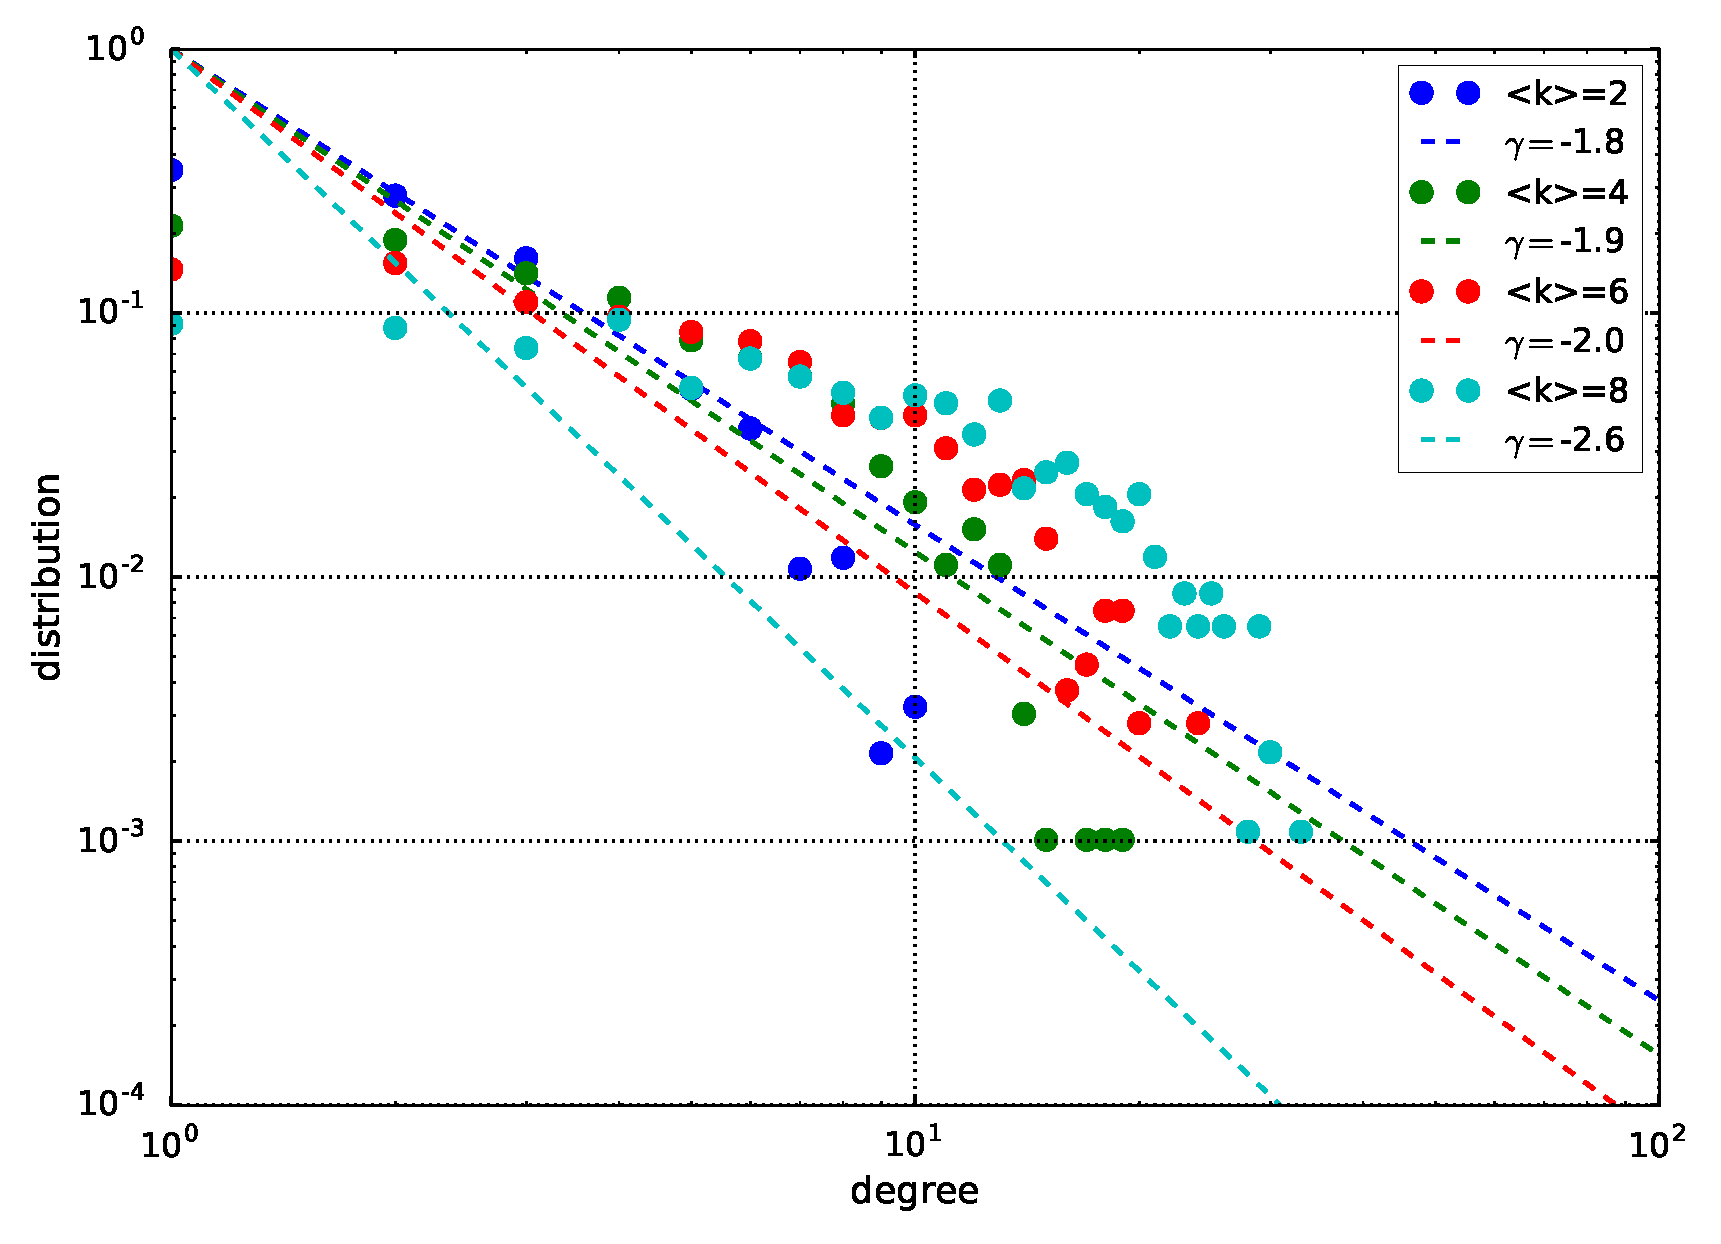
\includegraphics[width=10cm]{powerlaw_degree_dist.eps}
  \caption{Degree distribution of power law networks of $k=2,4,6,8$.
  The fitting curves are depicted by dotted lines.}
  \label{fig_degree}
\end{figure}

\section{Correlations between centrality metrics}
\label{centrality,option, corr}
As mentioned above, centrality metrics quantify node influence in a network based on varying mechanisms.
Here we first review the representative centrality metrics widely used.
\begin{itemize}

\item Degree(Deg)

Degree is the simplest and the most straightforward indicator to measure the importance
of certain individuals, that is, to count the number of vertices who have connected with it.
The presence of few highly connected hubs is the most prominent feature in terms of heterogeneity.
The vertices with the highest degree in the network usually are referred as hubs who
can influence more nodes effectively due to having the greatest number of neighbors.
Degree has been reported indeed play a crucial role in evolutionary games as well as in epidemic and propagation field.
For instance, players with a high degree possess evolutionary advantage due to the larger
number of games they play.
Therefore in the present work, Degree is seen as a fundamental metric in PD game.

\item Coreness(Cor)
The Coreness of a node is measured by k-core decomposition \cite{DorogovtsevGoltsev-18309} ,
which recursively pruning the nodes with degree less than current shell index and assigns each node with
an index $k_s$, representing its coreness in the network.
Recently, Kitsaket al. \cite{KitsakGallos-17826} argued that Coreness is a better indicator of a node’s
influence on spreading dynamics than Degree.
For example, if a hub exists at the end of a branch at the periphery of a network, it will have a minimal impact in the spreading process through the core of the network,
whereas a less connected person who is strategically placed in
the core of the network will have a significant effect that leads
to dissemination through a large fraction of the population.
This implies the topological position of individuals in population very likely affects evolutionary outcome.

\item H-index(Hid)

The Hirsch index (also called the H-index)\cite{Hirsch-18310} was originally used
to measure the citation impact of a scholar or a journal \cite{BraunGlänzel-18314}.
For a scholar or journal, the H-index is defined as the maximum value such
that there exists at least h papers, each with citation count.
Recently, H-index was extended to quantify the influence of users in social networks.
The H-index of a node is defined to be the maximum value such that there
exists at least $h$ neighbours of degree no less $h$.
Recently, Lü, L., et al.\cite{LüZhou-18192} indicated that Degree, H-index and Coreness are the initial, intermediate and steady states of the sequences, respectively;
and the H-index is a good tradeoff that in many cases can better quantify node influence than either
Degree or Coreness.

\item Betweenness(Bet)
Betweenness \cite{Anthonisse-18331} is one of the most popular geodesic-path-based ranking measures,
which is defined as the fraction of shortest paths between all node pairs that
pass through the node of interest.
It incorporates global information and is a simplified quantity for assessing the traffic carried by a
node.
L. Freeman \cite{Freeman-18315} has introduced the expression below to compute this centrality

\begin{equation}\label{Betweenness}
Bet(i)=\sum_{i\neq s,i\neq t,s\neq t}{\frac{g^i_{st}}{g_{st}}}
\end{equation}
where $g_{st}$ is the number of the shortest paths between $v_s$ and $v_t$
and $g^i_{st}$ is the number of the paths which pass through $v_i$
among all the shortest paths between $v_s$ and $v_t$.

\item Closeness(Clo)

The closeness \cite{KoschützkiLehmann-18332} of a node $i$ is the average hopcount
of the shortest paths from node i to all other nodes.
It measures how close a node is to all the others which based on information flow assumes that the shorter the distance a node from all other nodes, the faster the information disseminated.
Thus, the more central a node is the lower its total distance from all other nodes.
Closeness of node $i$ is computed by
\begin{equation}\label{closeness}
Clo(i)=\frac{N-1}{\sum_{j\in\mathcal{N}\backslash{i}}{H_ij}}
\end{equation}

where $H_ij$ is the hopcount of the shortest path between nodes $i$ and $j$,
and $\sum_{j\in\mathcal{N}\\{i}}{H_{ij}}$ is the sum of the hopcount of the shortest paths from
node $i$ to all other nodes.

\item Clustering(Clu)

Clustering Coefficient(CC) was proposed by Duncan J. Watts and Steven Strogatz \cite{WattsStrogatz-18333} in order to determine whether a graph is a small-world network.
For a node $i$, the local clustering coefficient $C$ is the fraction of actual links within its neighborhood to the number of potential links that could possibly exist among them.
In a different context the clustering coefficient characterizes the proportion between the number of observed triangles to all possible triangles as link transitivity in one network, quantifying how close its neighbors are to being a clique (complete graph).
In many cases the presence of clustering structure in the network seems to be the crucial feature responsible for favoring cooperators or defectors\cite{SantosPacheco-18280,HuangZheng-18221}.
In the context of evolutionary dynamic, it is reasonable to quantify the influence of a node through its clustering coefficient.
Notice that CC takes smaller values for more central nodes, which is in opposite to the other centrality measures, whereas we still rank individual importance by CC values which will unveil the effect of non-importance.

\item Eigenvector(Eig)
Eigenvector centrality supposes that the influence of a node is not only determined by the number of its neighbors, but also determined by the influence of each neighbor.
The centrality of a node is proportional to the summation of the
centralities of the nodes to which it is connected.
Its variant, Google's PageRank based on the concept that connections to high-scoring sites contribute
more to the score of the site in question than equal connections to low-scoring sites, is more well-known.
The Eigenvector centrality of node $i$ is
\begin{equation}\label{Eigenvecotr}
Eig(i)=\frac{1}{\lambda}\sum_{j=1}^{n}{Eig(j)}
\end{equation}

where $\lambda$ is the largest eigenvalue of adjacent matrix of network.

\end{itemize}

\label{centraltiy correlation}
    Although the correlations between centrality metrics have been studied\cite{LiLi-18181,šikićLančić-17843},
the ranked sequence of vertices heavily depends on the dynamical regime and the topological features of network.
It is necessary to investigate the correlation between any two centrality metrics on
the networks used in the present study.
As detailed in Fig.\ref{fig corr centrality k=2} and \ref{fig corr centrality k=8}, we computed the Pearson correlation coefficients between any two centrality metrics in networks of $k=2$ and $k=8$ separately.
    On the one hand, the outcomes indicate that strong linear correlations do exist
between certain centrality metrics such as Degree and Eigenvector, Degree and Betweenness, H-index and Closeness, particularly which are strongly positive correlated(Pearson correlation coefficients >0.9) in the case of $k=8$.
It is natural to expect they maybe have akin influence in evolutionary dynamic.
    On the other hand, the density of connections among population, denoted by $k$, impacts
distributions and correlations of certain centralities.
In sparse network due to lacking enough connections, most nodes have identical centrality values
thus it is more difficult to distinguish different individuals through centralities.
Accordingly, the correlations of different centralities also weaken.


\begin{figure}
  \centering
  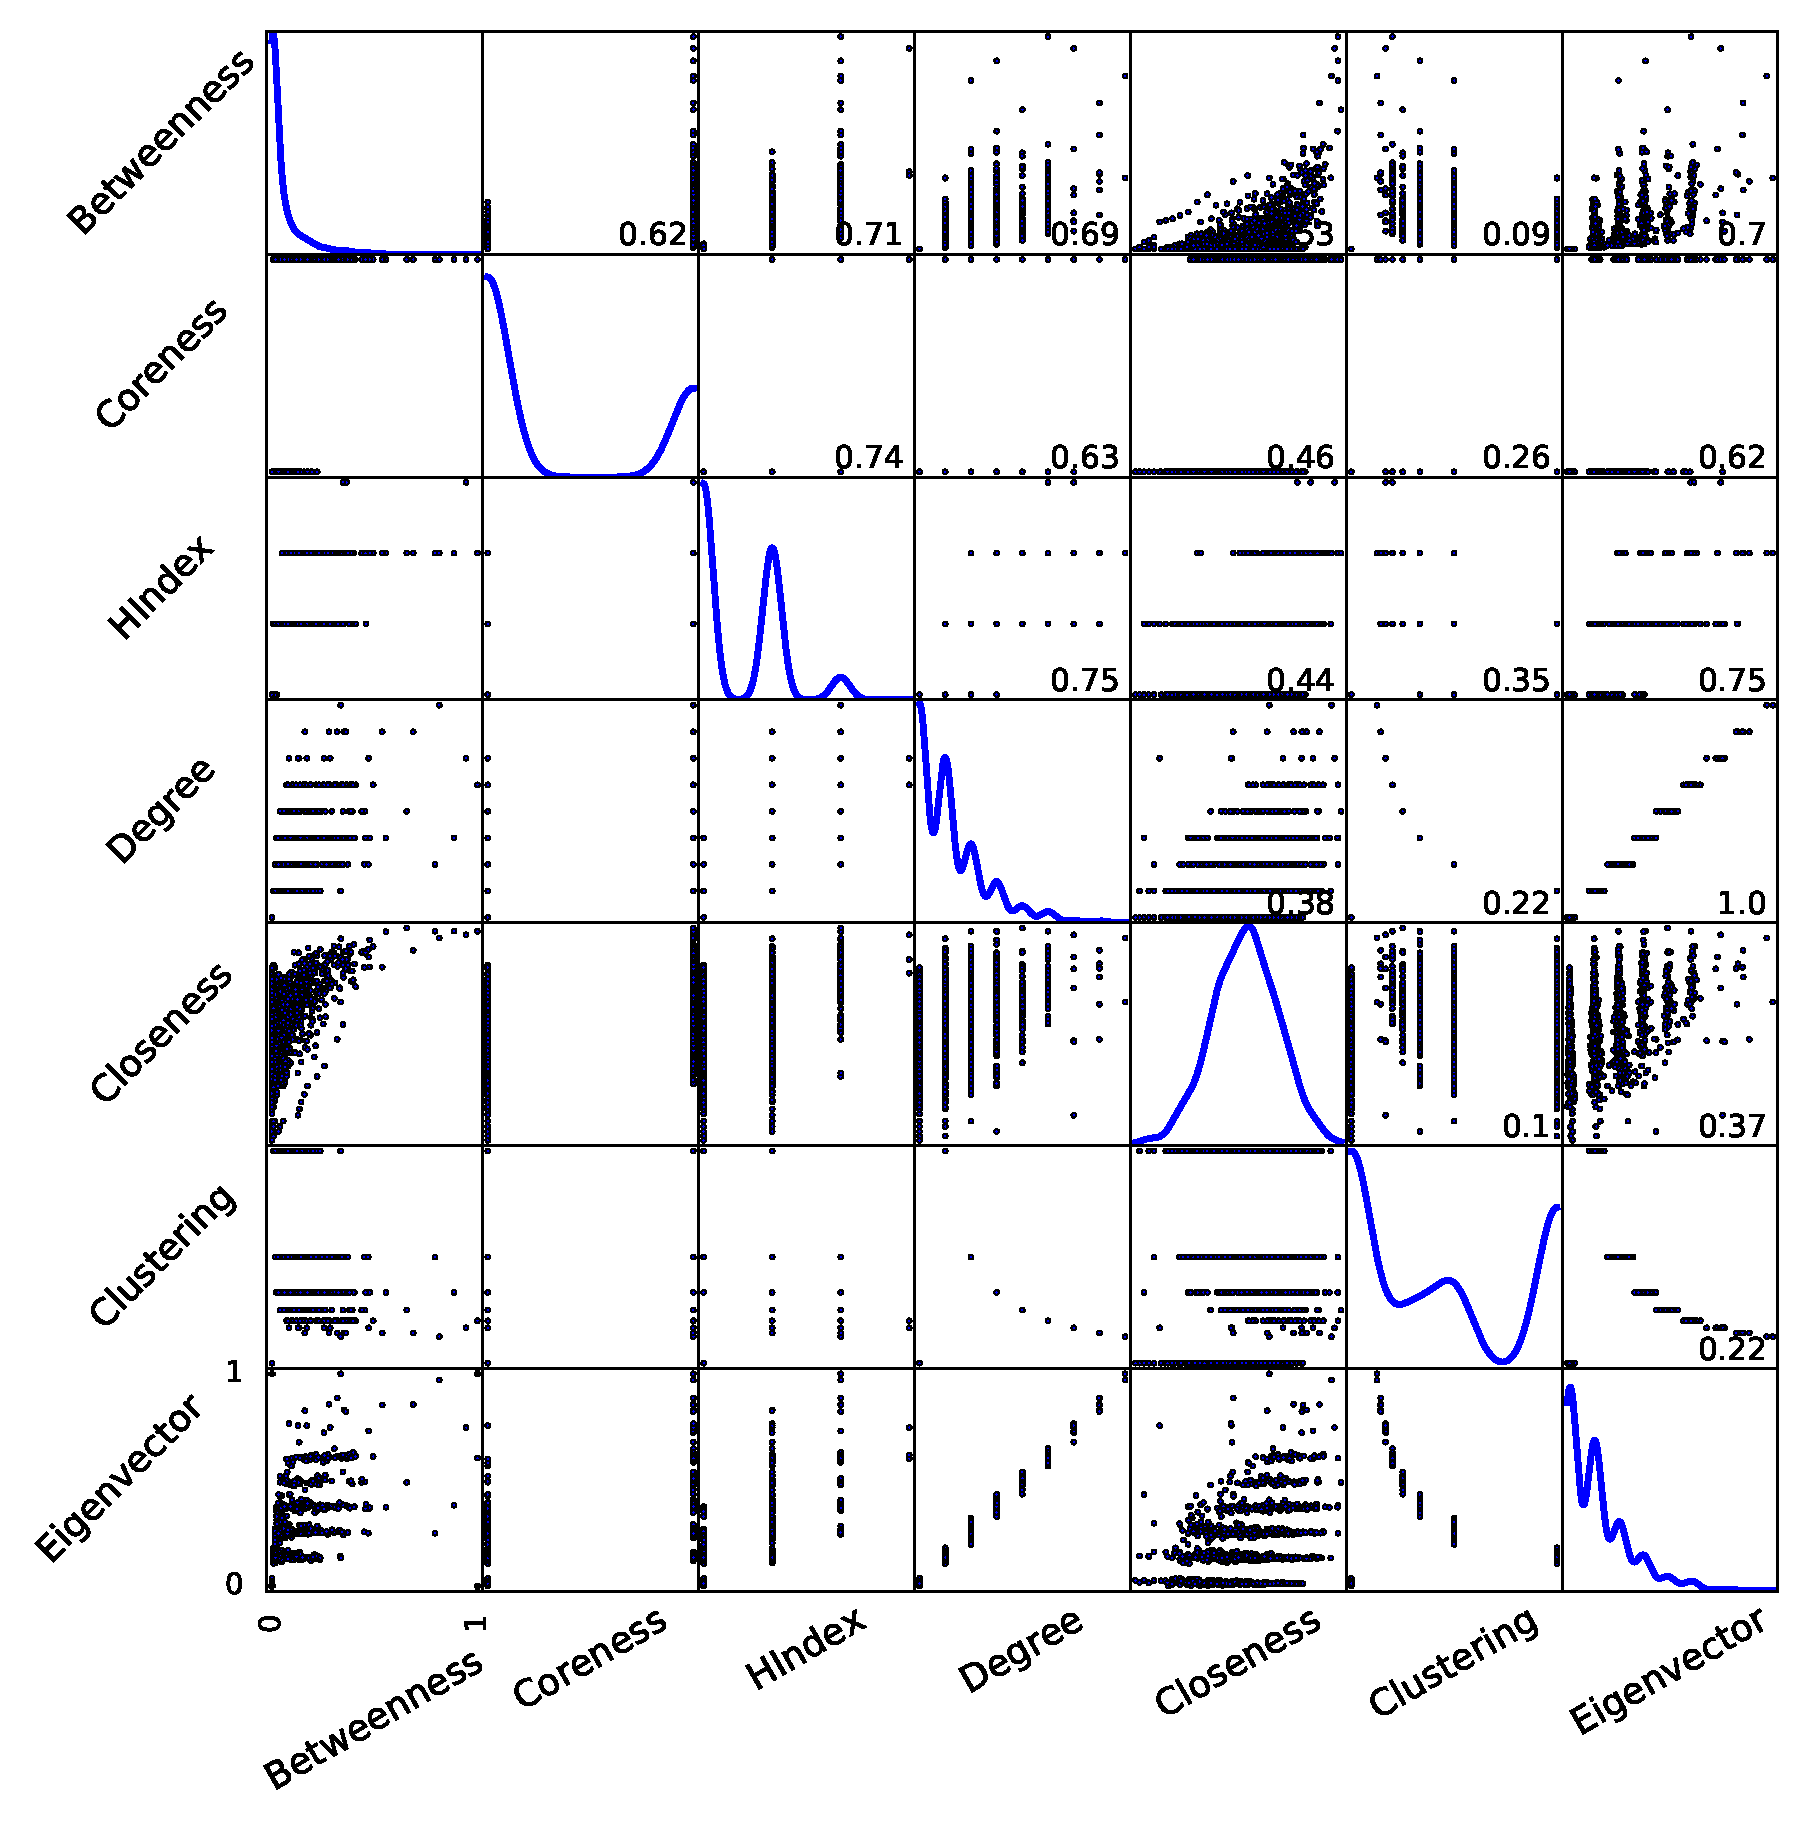
\includegraphics[width=16cm]{Powerlaw_k2_centrality_correlation.eps}
  \caption{Correlation matrix and distributions of centralities considered in this study on network of $k=2$.
  The diagonal insets depict density estimation of centralities.
  The Pearson Correlation Coefficients of any two centrality metrics are shown on upper triangular insets.
  Note that the centrality Eigenvector and Degree indicates a perfect positive correlation.
  It also should be noted that centrality Clustering is negatively correlated with all the other centralities.
    }
  \label{fig corr centrality k=2}
\end{figure}

\begin{figure}
  \centering
  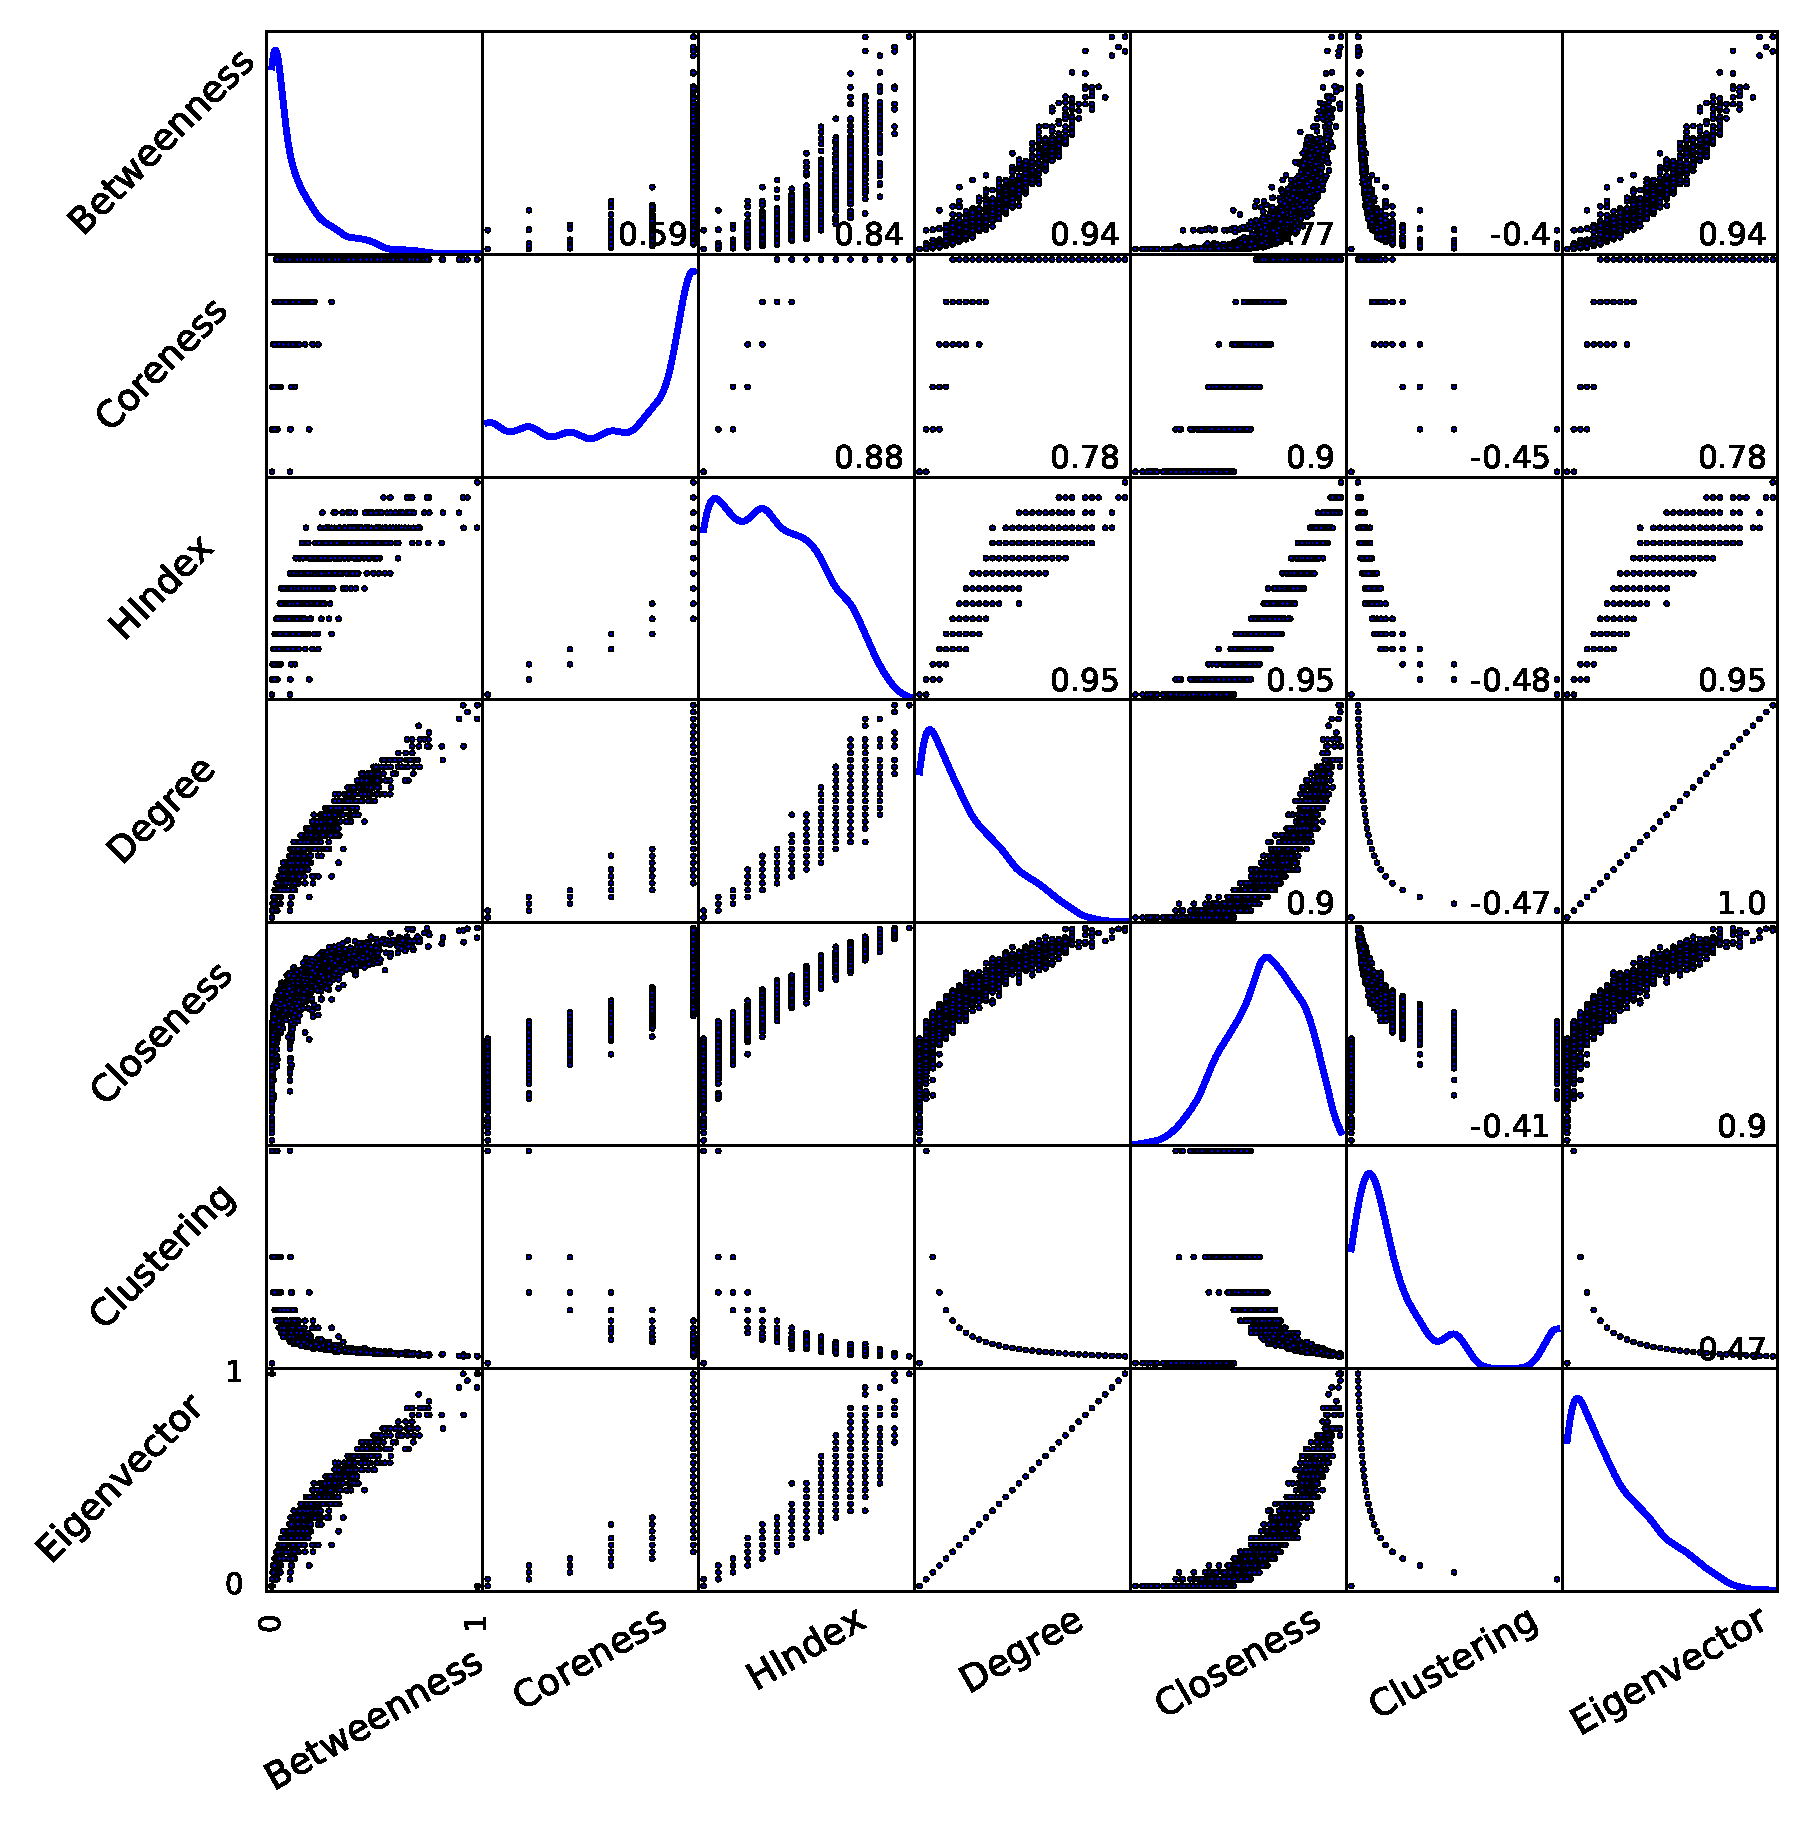
\includegraphics[width=16cm]{Powerlaw_k8_centrality_correlation.eps}
  \caption{Correlation matrix and distributions of centralities considered in this study on network of $k=8$.
  }
  \label{fig corr centrality k=8}
\end{figure}



%%%%%%%%%%%%%%%%%%%%%%%%%%%%%%%%%%%%%%%%%%%%%%%%%%%%%%%%%%%%%%%%%%%
\section{ Results and discussion}

\subsection{Benchmark simulation}

    The presentation of the results begins with the standard imitator dynamics
on a series of scale-free networks which would be seen as benchmark for the following further results.
Fig.\ref{powerlawK2468TSPanel} illustrates the impact of average degree $k$
and initial proportion of cooperators $\rho_C(0)$ on the outcome of the T-S space panel.
    In the first place, it is clearly evidenced that heterogeneity boosts cooperation
as verified in previous works, albeit there are arguments in experiments on this point as for example Carlos Gracia-Lázaro, etl \cite{Gracia-LázaroFerrer-18206} argue that heterogeneous networks do not promote cooperation when humans play a Prisoner’s Dilemma.
Under the present conditions, we confirmed the effect of heterogeneity for driving cooperation.
    Second, the area of full cooperation in the T-S panel is extended with the
increase of $\rho_C(0)$, which indicates that the stable cooperation level largely depends on the initial condition, the importance of which was underestimated even was ignorant in previous works.
    And finally, it is suggested that with the average degree increasing the networks
approximates more and more closely to the well-mixed structure, which has been proved to be inhibitor toward cooperators.
Consequently,the populations of larger $k$ would lead to the lower cooperation level.
However, it can be observed that the influence of $k$ is not monotonous toward cooperation level,
k=2 being the exception from k=4,6,8.
We therefore further inspect the conditions of smaller resolution of $k$ and the result is given
in Fig.\ref{powerlawK23TSPanel}.
Fig.\ref{powerlawK2468TSPanel} and Fig.\ref{powerlawK23TSPanel}
show that irrespective of initial fraction of cooperators the mean $\rho_{c}(\infty)$ on T-S panel reaches the maximum at $k=2.7$.
In other words, the cooperation level does not monotonously depend on the average degree of underlying network, existing an intermediate connection density optimally sustaining cooperation.


\begin{figure}[htbp]
\centering
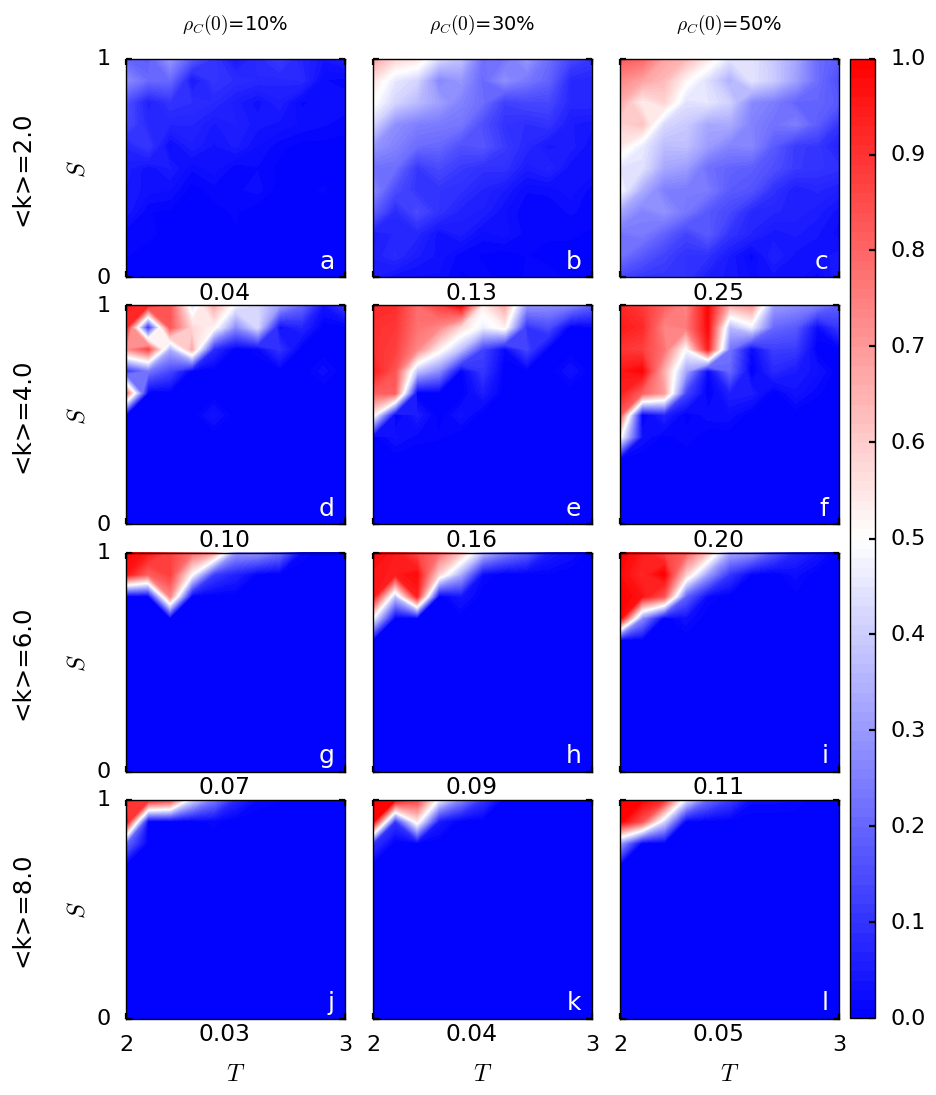
\includegraphics[width=12cm]{powerlawK2468TSPanel.png}

\caption{\cooplevel.
The average degrees of networks cover $k=2(a,b,c),4(d,e,f),6(g,h,i),8(j,k,l)$.
The update rule is Fermi imitation and he initial densities of cooperators are:
$\rho_{C}(0)=0.1,0.3,0.5$(columns from left to right).
The presented results indicate that the evolution of cooperation is affected by initial condition and degree.
Note the non-monotonicity of the results dependent on degree $k$.}
\label{powerlawK2468TSPanel}
\end{figure}

\begin{figure}[htbp]
\centering
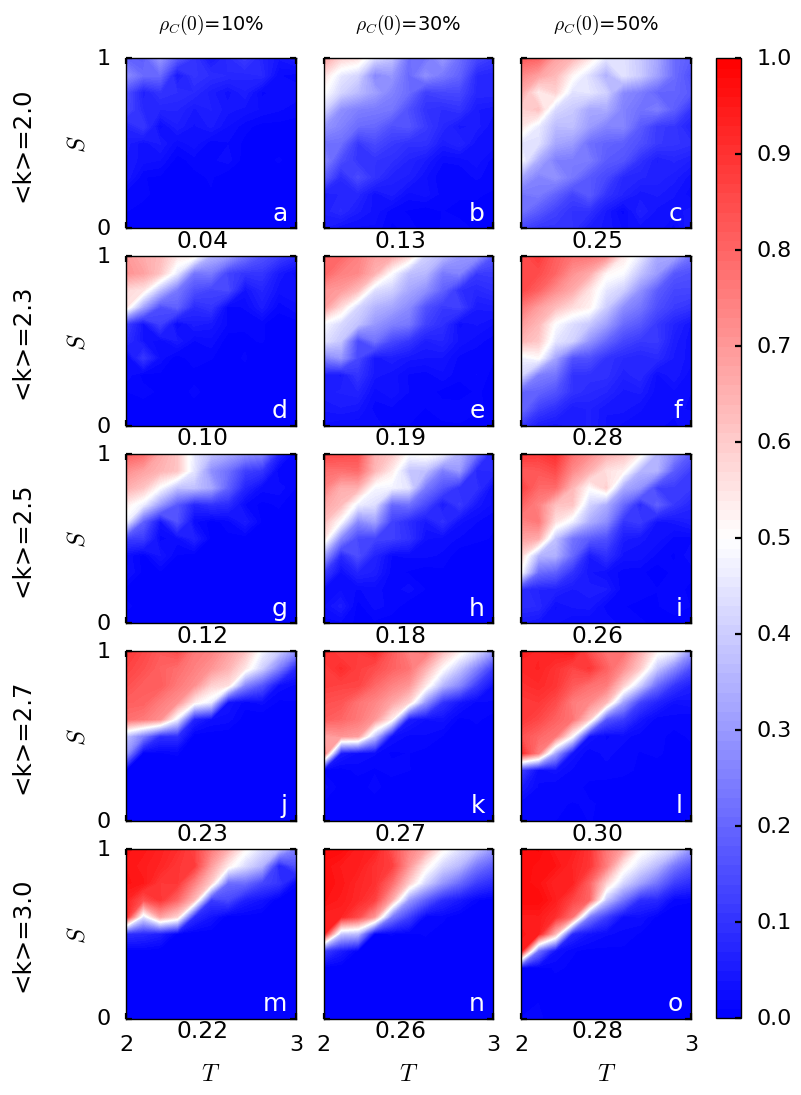
\includegraphics[width=12cm]{powerlawK23TSPanel.png}

\caption{Asymptotic density of cooperators $\mathcal{C}$ on the T-S plane.
The average degrees of networks cover $k=2(a,b,c),2.3(d,e,f),2.5(g,h,i),2.7(j,k,l)$, 3.0(m,n,o).
Other parameters are the same as in Fig.\ref{powerlawK2468TSPanel}.
This result evidences cooperation can be optimally promoted in the degree between 2.5 and 3.0.}
\label{powerlawK23TSPanel}
\end{figure}


\subsection{Centrality preferential cooperators}
%%% top rank cooperator

    In this section, we proceed exploring the evolution of cooperation considering non-random strategy assignment.
In our simulations, all the players are ranked in terms of a centrality metric then pickup top-p players as cooperators,
namely the initial faction of cooperation $\rho_c(0)=p/N$.
    In what concerns the initial conditions, we discuss this
setup for two main reasons.
    1)Complete random assignment of strategy, one of default setups in many previous
researches, does not always consist with real-world conditions since individuals generally have more or less preferences and consider comprehensive factors when take action in evolutionary dynamics.
To say the least, the evolutionary dynamic will proceed into non-random state even initiates from random condition.
    2)Stimulating importance individuals to cooperate is a feasible and applicable approaches in the purpose of promoting cooperation.

    The results based on the setups above for $k=2,2.7,4,8$ are depicted separately
in Figs.\ref{PowerlawK2TopRankTSPanel}, \ref{PowerlawK2.7TopRankTSPanel},
\ref{PowerlawK4TopRankTSPanel}, and \ref{PowerlawK8TopRankTSPanel}.
Notably, we have assessed the conditions where $k=2~3$ at interval 0.1 and $k=3~8$ at interval 1,
while only present the representative results corresponding to the benchmark simulations \ref{powerlawK2468TSPanel}and \ref{powerlawK23TSPanel}.
    On the whole, preferential initialization significantly promotes cooperation in the region of T-S space
compared with the random cases, which happens irrespectively of the values of initial fraction of cooperators and, more importantly,
of the degree $k$.
All the centralities give some degrees of boost for cooperation and
as predicted in the section before the sole exception that deviates others is Clustering.
    Fig.\ref{PowerlawK2TopRankTSPanel} displays the simulation result in sparse network $k=2$,
corresponding to the benchmark of first row in Fig.\ref{powerlawK2468TSPanel}.
To compare the effect of different centralities, we rank centralities according to $\mathcal{C}$
and sensitivity to $\rho_{C}(0)$ as following

\begin{eqnarray*}
\left\{
\begin{aligned}
\mathcal{C}_{Deg}>\mathcal{C}_{Bet}>\mathcal{C}_{HIn}>\mathcal{C}_{Clo}>\mathcal{C}_{Cor}>\mathcal{C}_{Clu}  \qquad \rho_{C}(0)=0.1,\\
\mathcal{C}_{Bet}>\mathcal{C}_{Deg}>\mathcal{C}_{Cor}>\mathcal{C}_{Hin}>\mathcal{C}_{Clo}>\mathcal{C}_{Clu}  \qquad \rho_{C}(0)=0.3,\\
\mathcal{C}_{Bet}>\mathcal{C}_{HIn}>\mathcal{C}_{Deg}>\mathcal{C}_{Cor}>\mathcal{C}_{Clo}>\mathcal{C}_{Clu}  \qquad \rho_{C}(0)=0.5.
\end{aligned}
\right.
\end{eqnarray*}

Basically, the centralities can be roughly classified into two groups according to relative sequence.
It can be observed that Betweenness, Degree and HIndex can noticeably enhance the resilience of cooperation
compared with others, especially in the case of $\rho_{C}(0)=0.1$(see the first column).
However, all the centrality can not hold stabilization toward the variation of $\rho_{C}(0)$, depending sensitively on it.
As increasing $\rho_{C}(0)$, the gaps of $\mathcal{C}$ between different centralities reduce,
which attributes to the power law distribution of centrality of vertices(see Fig.\ref{fig corr centrality k=2}).
Another distinctive evolutionary feature in sparse network is the coexist of cooperators and defectors in certain
region of T-S plane, particularly for the centrality Closeness(panels d,e,f) and Coreness(panels j,k,l)
that cannot yield full-cooperation($\mathcal{C}=1$) on the T-S plane.
    Results for the degree $k=2.7$ are reported in Fig.\ref{PowerlawK2.7TopRankTSPanel}.
As plots clearly show, the overall level of cooperation in this case considerably outperform that of $k=2.0$
as well as in the benchmark results.
Similarly, centrality Degree, Betweenness and HIndex still play the role of better promotors and Closeness, Coreness, Cluster play worse one, but the discrepancy weakens.
In addition, the sensitivity of each centrality toward initial condition also alleviate.
    Fig.\ref{PowerlawK4TopRankTSPanel} corresponds to the case of degree $k=4$.
The overall $\mathcal{C}$ of each panel is similar as the case of $k=2.7$,
which is inconsistent with the influence of degree $k=2.7$(Figs.\ref{powerlawK23TSPanel}j,k,l)
and $k=4$(Figs.\ref{powerlawK2468TSPanel}d,e,f) in the benchmark result.
Meanwhile, the all-cooperator phase and all-defector phase occupy the T-S plane and the
boundary of their transition become evident.
In the case of $k=8$ illustrated in Fig.\ref{PowerlawK8TopRankTSPanel},
a similar situation is observed, albeit the cooperation level slightly declines.
    Another noteworthy outcome is that with the rise of degree $k$, the transition boundary between
all-cooperator and all-defector gradually deviate the parallel of diagonal line in the T-S plane.
For example as displayed in Fig.\ref{PowerlawK8TopRankTSPanel}c, the cooperation density
$\rho_{c}(\infty)=1$ when $T<0.45$ regardless of the variation of $S$, accordingly larger than which cooperators almost vanish.


\begin{figure}[htbp]
\centering
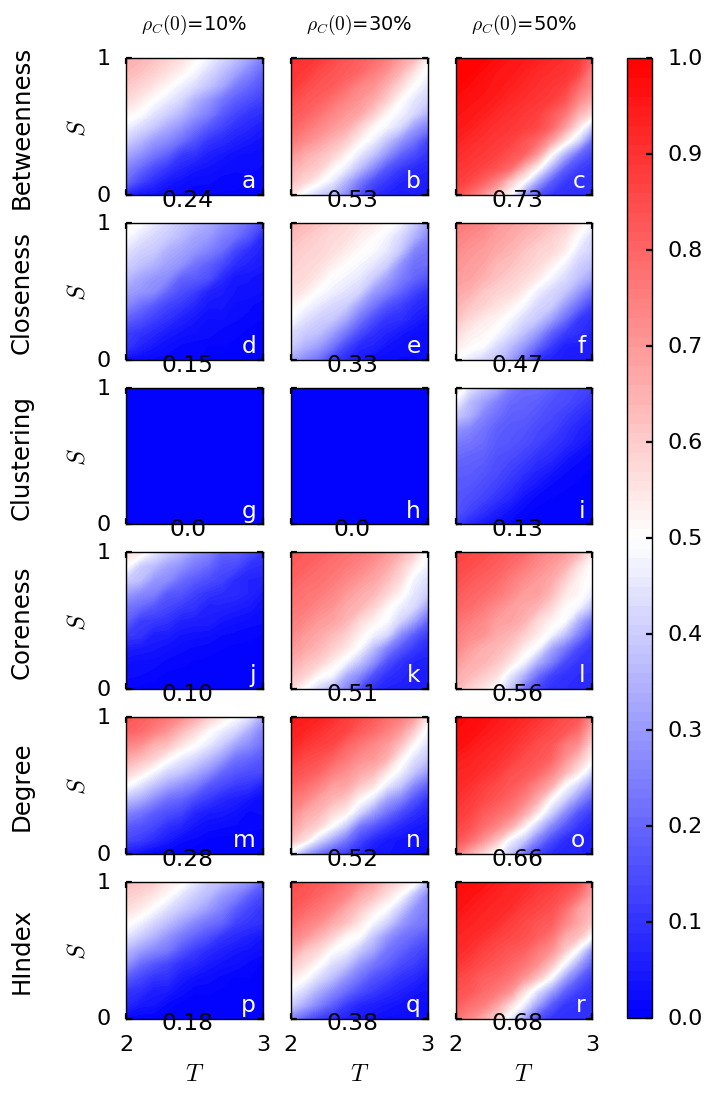
\includegraphics[width=13cm]{PowerlawK2TopRankTSPanel.png}

\caption{Asymptotic density of cooperators $\mathcal{C}$ in degree $k=2$.
Comparing with the baseline case(see Fig.\ref{powerlawK2468TSPanel}a,b and c),
the evolution of cooperation is substantially promoted.
}
\label{PowerlawK2TopRankTSPanel}
\end{figure}


\begin{figure}[htbp]
\centering
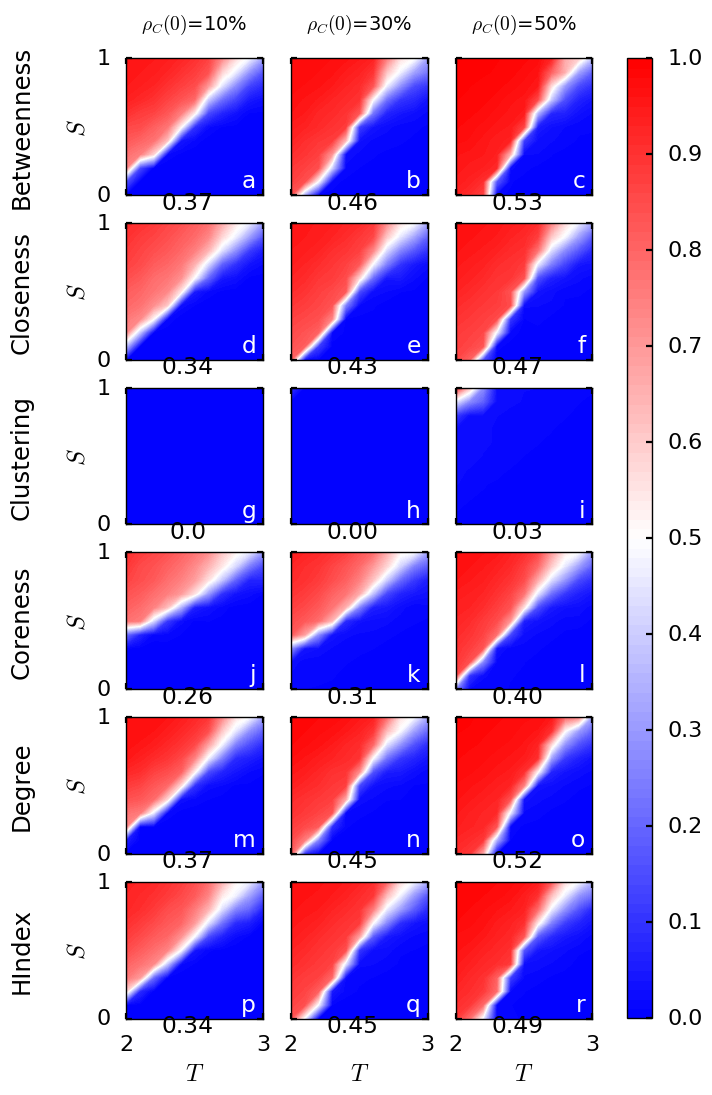
\includegraphics[width=13cm]{PowerlawK2.7TopRankTSPanel.png}

\caption{Asymptotic density of cooperators $\mathcal{C}$ in degree $k=2.7$.
Comparing with the baseline case(see Fig.\ref{powerlawK2468TSPanel}a,b,c) and
degree $k=2.0$(see Fig.\ref{PowerlawK2TopRankTSPanel}),
the evolution of cooperation is optimally promoted regardless of initial condition and centralities.}
\label{PowerlawK2.7TopRankTSPanel}
\end{figure}


\begin{figure}[htbp]
\centering
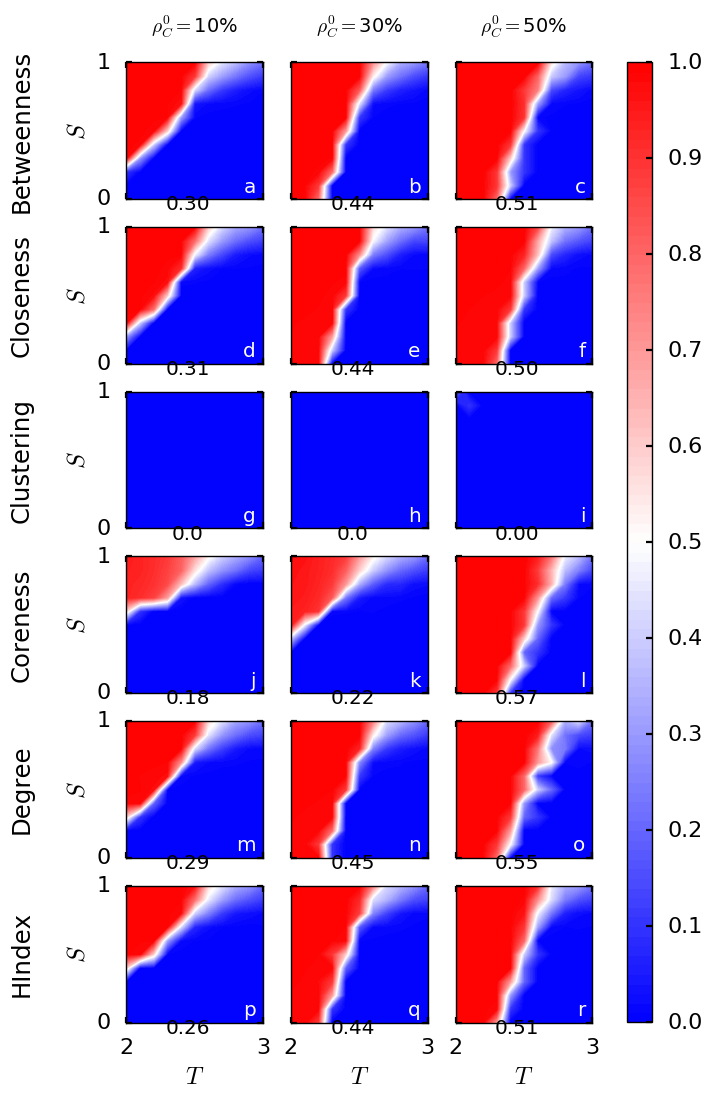
\includegraphics[width=13cm]{PowerlawK4TopRankTSPanel.png}

\caption{Asymptotic density of cooperators $\mathcal{C}$ in degree $k=4$.}
\label{PowerlawK4TopRankTSPanel}
\end{figure}


\begin{figure}[htbp]
\centering
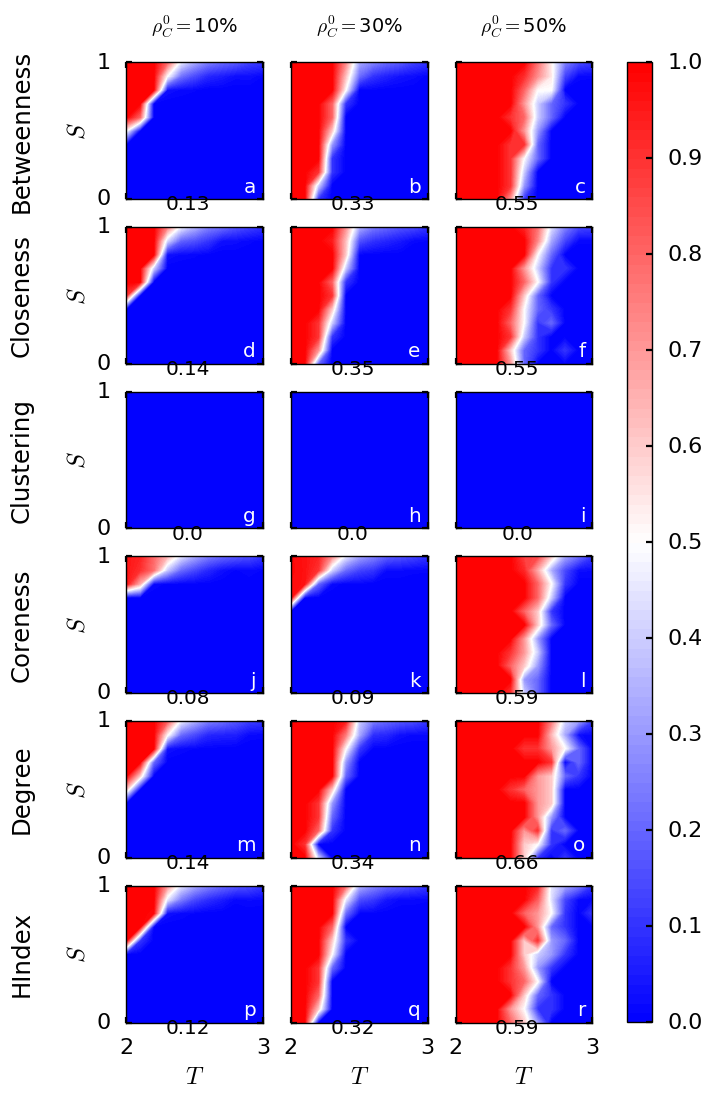
\includegraphics[width=13cm]{PowerlawK8TopRankTSPanel.png}

\caption{Asymptotic density of cooperators $\mathcal{C}$ in degree $k=8$.}
\label{PowerlawK8TopRankTSPanel}
\end{figure}

\begin{figure}[htbp]
\centering
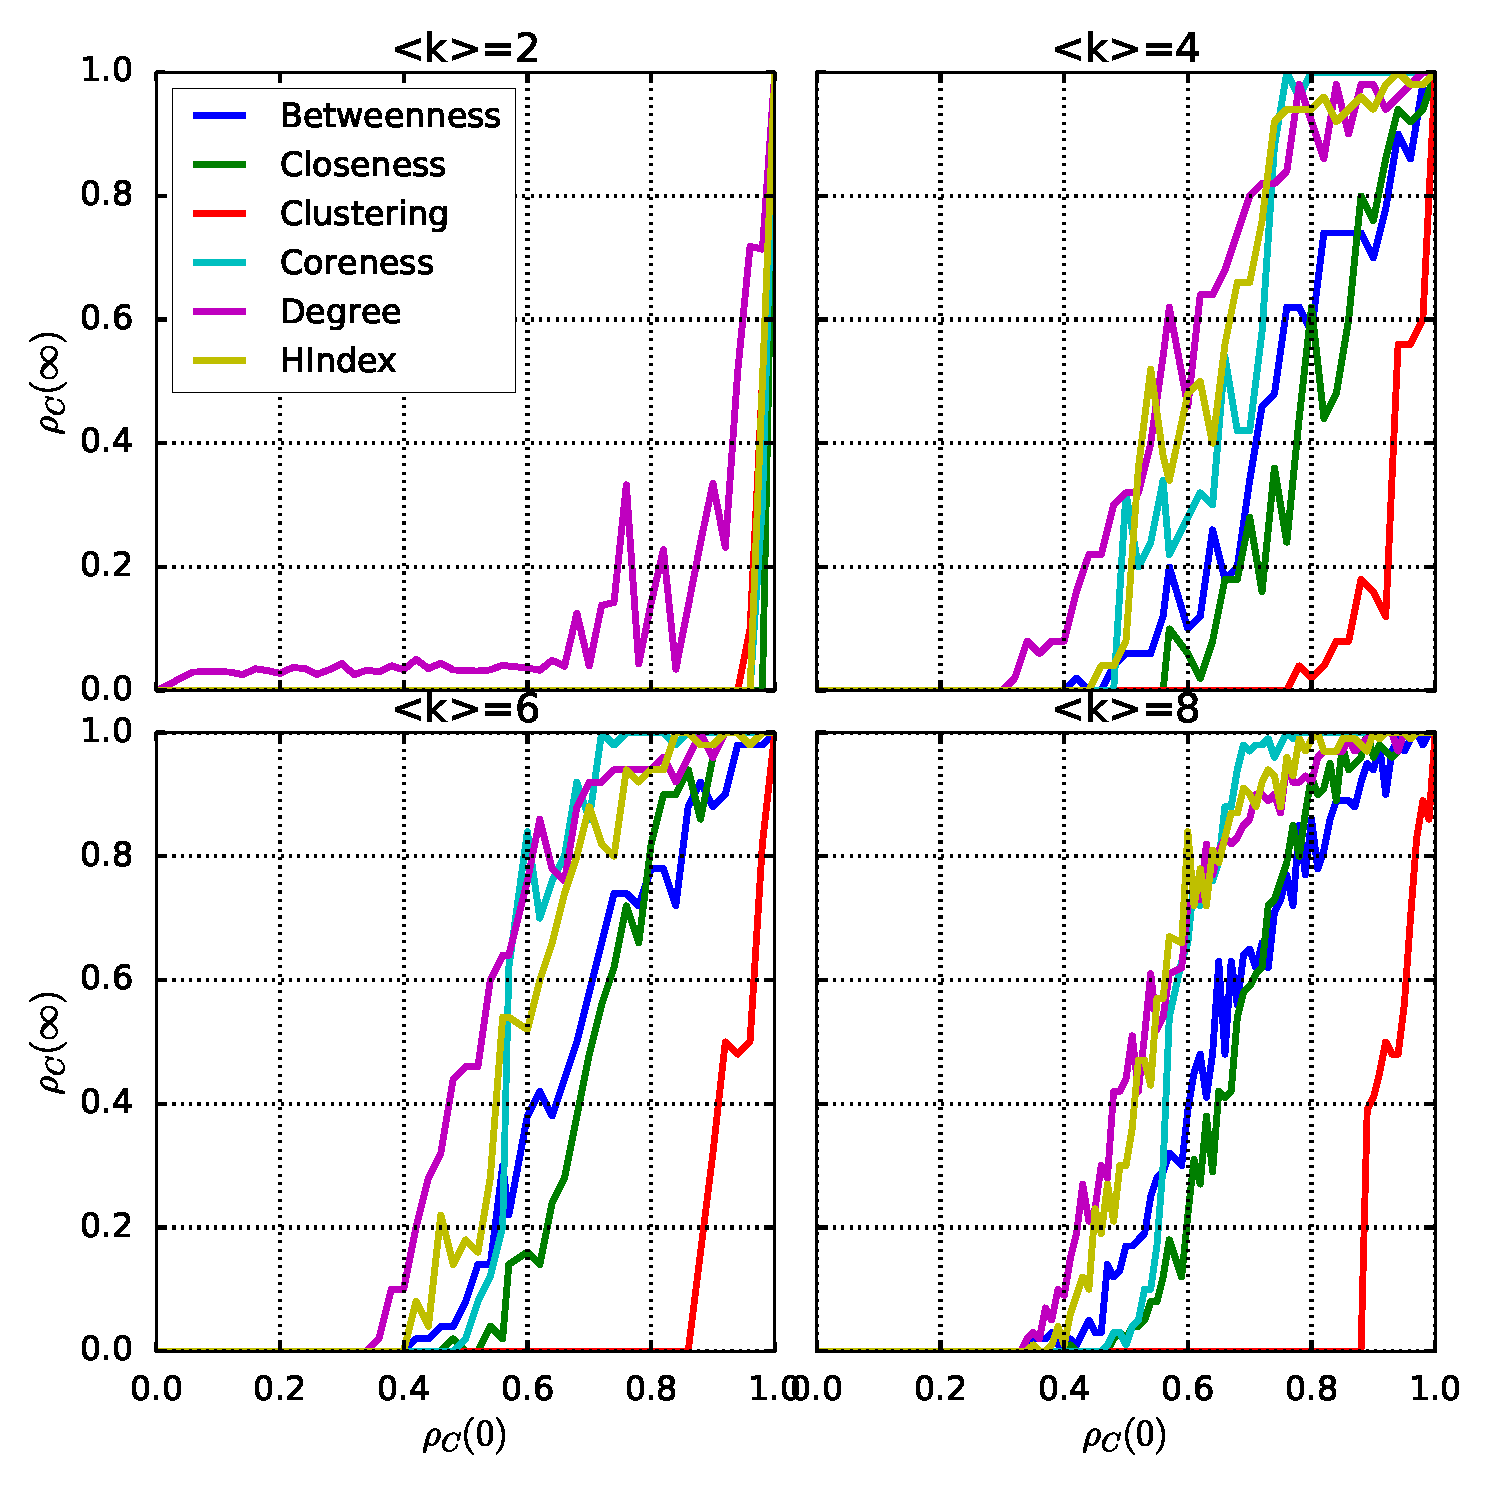
\includegraphics[width=10cm]{init_vs_stable_coop_density.eps}

\caption{The final cooperation level as function of initial cooperation level.
T=2.5,S=0.2. sample by 0.02. }
\label{InitVsFinalCoopLevel}
\end{figure}



\subsection{Payoff and centrality mixed update strategy} %%%  centrality update strategy
    All the results presented so far have been obtained with a standard Fermi imitator
update of strategies, namely the payoff based evolutionary dynamic.
Previous research, supported in theoretical\cite{CiminiSanchez-18359} and experimental\cite{Gracia-LázaroCuesta-18325} results, suggests that absence of network reciprocity is a general feature of evolutionary dynamics if players do not base their decisions on others’ payoffs.
What's the result if population consider non-payoff and payoff-centrality mixed based evolutionary dynamic?
    To simulate these cases, the Fermi imitator probability Eq.(1) is replaced by
payoff and centrality mixed version

\begin{equation}
\mathcal{P}(s_y^t\rightarrow s_x^{t+1})=max\{ \frac{1}{1+e^{-[(P_y^t-P_x^t)]/k}},\frac{1}{1+e^{-[(C^i_y-C^i_x)]/k} }\}
\label{eq_mixedFermi}
\end{equation}
where $C^i_x$ indicates player x's score of centrality $i$.

    Here the update rule incorporates the affection of individual centrality by comparing both payoffs
and centralities so that the final probability is stochastically determined by the pairwise ones with higher gap.
    If the term $1+e^{-[(P_y^t-P_x^t)]/k}$ is removed from Eq.\ref{eq_mixedFermi},
the dynamic becomes non-payoff update rule.
Perceptibly, it ought to yield overall full cooperation results in the present simulation.
Because the player's centrality keep invariant, together with the initial cooperators possess larger centrality scores, the imitation of strategy is unidirectional, which implies that the defectors with lower
centrality definitely replicate the cooperation strategy but not vice versa.
Therefore, we focus attention to the mixed condition.
    Intuitively, one might assume introducing centrality into mixed strategy updating
will improve the cooperation level as well as in the case of aforementioned non-payoff update,
at least non-worse outcomes.
Rather contrary, as shown in Figs.\ref{PowerlawK2RankUpdate}~\ref{PowerlawK8RankUpdate} it is clear that, compared with traditional Fermi update network reciprocity fails to protect cooperators.
Comparing Fig.\ref{PowerlawK2RankUpdate} and Fig.\ref{PowerlawK2TopRankTSPanel},
for example, represents the dramatic difference between payoff-based and mixed-based updating strategy
on degree $k=2$ where besides centrality Degree(panels m,n and o in Fig.\ref{PowerlawK2RankUpdate}),
the other cooperation densities drop to almost zero.
    To elucidate this paradox phenomenon, we examine two realizations of simulations based on
payoff update and mixed update separately.
Without loss generality, we choose the parameter values of $k=4,T=2.5,S=0.5,\rho_{C}(0)=0.3$
and Closeness centrality.
    The sharp differences in results is clearly shown in Fig.\ref{payoffUpdateProcess}(payoff update)
and Fig.\ref{centralityUpdateProcess}(mixed update).
Panel (d) plots the frequency of switching between cooperators and defectors of each player,
which presents identical characteristic between payoff and mixed update rules.
The frequency of switching is stronger heterogeneity in Fig.\ref{payoffUpdateProcess}d compared with that in Fig.\ref{centralityUpdateProcess}d.
Despite all the players update strategy in the similar frequency in mixed update rules, there are no
update-stable ones.
    Another noticeable difference is the players with higher centralities are more stable, namely seldom change
strategy.

    This result, apparently caused by the mixed update, drives us to further investigate individual
behaviors in order to clarify the underlying causes.
According to the mixed update rule Eq.\ref{eq_mixedFermi}, there are four possible situations regarding of payoff and centrality when a player x as imitator intends to change strategy:
\begin{eqnarray}
\left\{
\begin{aligned}
(a)\qquad C_x<C_y,P_x<P_y,\\
(b)\qquad C_x>C_y,P_x<P_y,\\
(c)\qquad C_x<C_y,P_x>P_y,\\
(d)\qquad C_x>C_y,P_x>P_y,
\end{aligned}
\right.
\label{eq_mixedupdate_conditions}
\end{eqnarray}
where $C_x$ and $C_y$ indicate the centrality of imitator and imitated player separately.
    Based on Fermi Function, Imitator x explicitly prefers to update strategy in condition (a)
and to retains strategy in condition (b).
That is to say, payoff and centrality induce player to take unanimous behavior,
but which is opposite in conditions (b) and (c).
    Accordingly, we calculated the numbers of update behaviors determined by payoff and centrality
and corresponding numbers of conditions (b) and (c).
Fig.\ref{centralityUpdateProcessDetails} presents this in two patterns of strategy updating separately,
Cooperation to Defection(panel a) and inverse case(panel b).

Note that
which gives rise to the probability
$1+e^{-[(P_y^t-P_x^t)]/k}$
$1+e^{-[(C^i_y-C^i_x)]/k}$
In the following we also consider the case of normalized payoffs.

Because players' centrality scores are normalized to [0,1] but payoffs not, most update behaviors arise from comparing payoffs.


Those players with highest centralities obtain larger payoffs hence they have no incentive to change strategy.
However, for majority players with small centralities,



We also validate the case of normalized payoffs, it doesn't qualitatively alter above result.


\begin{figure}[htbp]
\centering
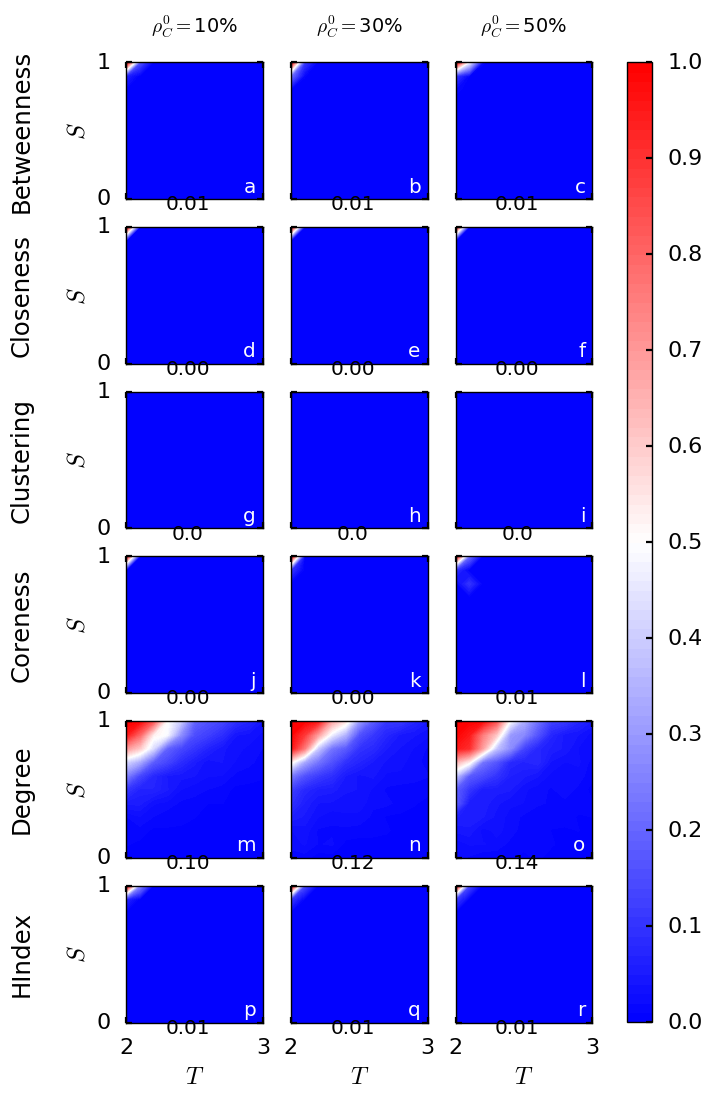
\includegraphics[width=13cm]{PowerlawK2RankUpdate.png}
\caption{Asymptotic density of cooperators $\mathcal{C}$ in degree $k=2$.
The initial condition is centrality favored cooperator and the update rule is Centrality imitation.
Other parameters are the same as in Fig.\ref{powerlawK2468TSPanel}}
\label{PowerlawK2RankUpdate}
\end{figure}


\begin{figure}[htbp]
\centering
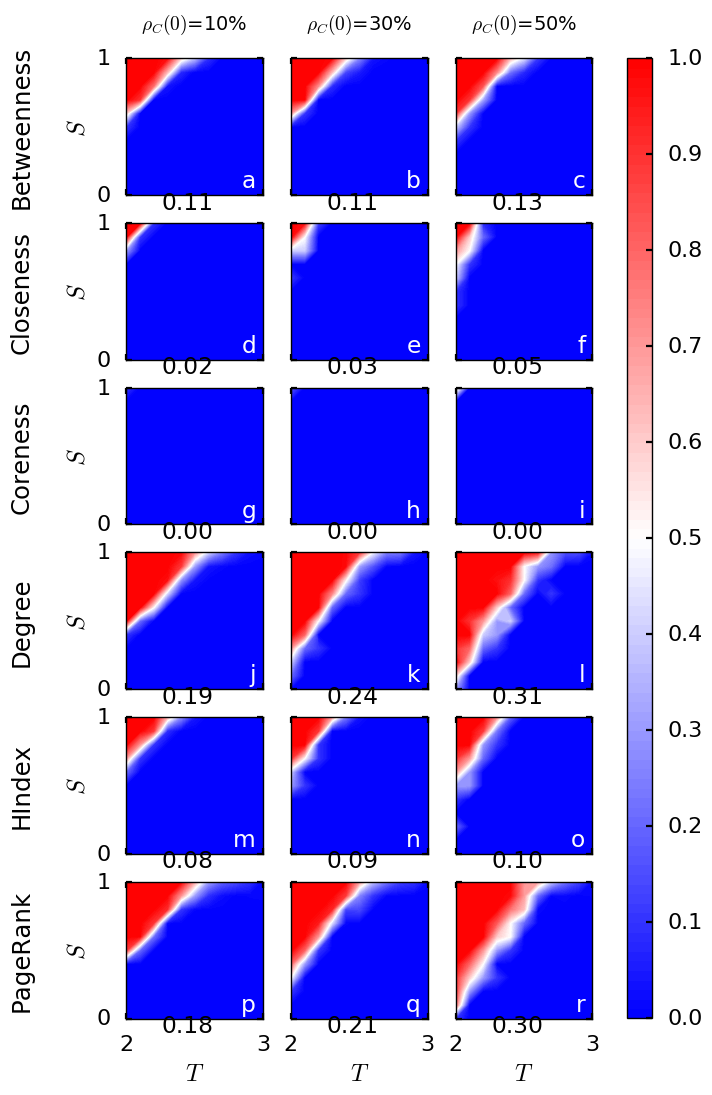
\includegraphics[width=13cm]{PowerlawK2.7RankUpdate.png}
\caption{Asymptotic density of cooperators $\mathcal{C}$ in degree $k=2.7$.
Other parameters are the same as in Fig.\ref{PowerlawK2RankUpdate}.}
\label{PowerlawK2.7RankUpdate}
\end{figure}

\begin{figure}[htbp]
\centering
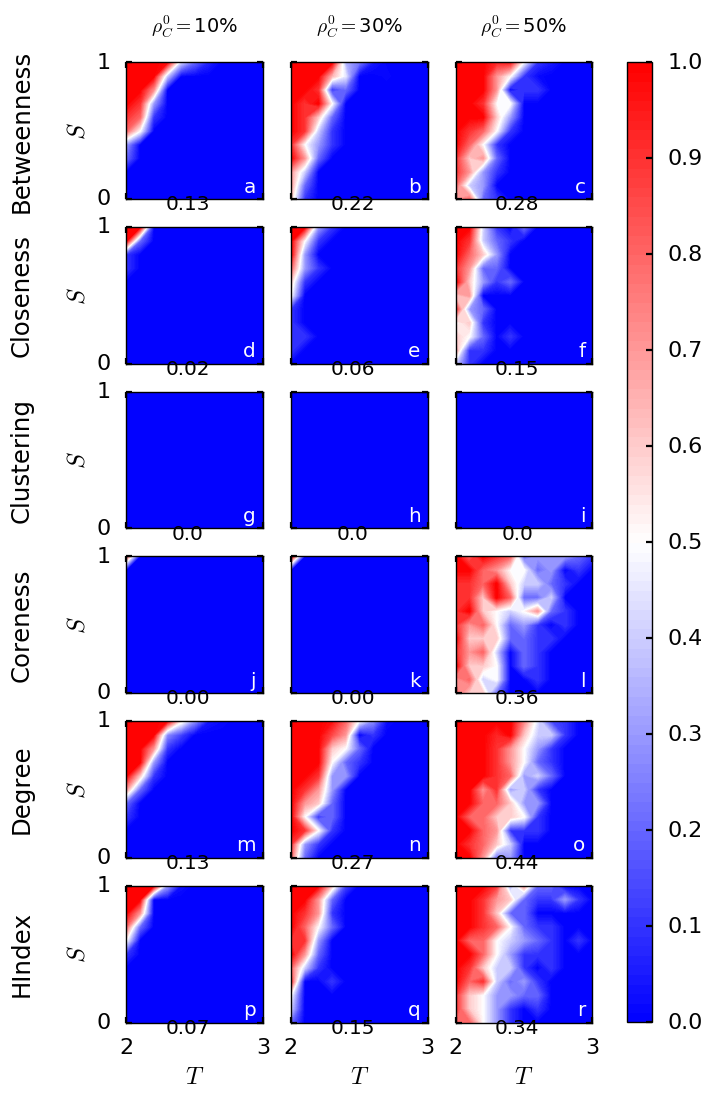
\includegraphics[width=13cm]{PowerlawK4RankUpdate.png}
\caption{Asymptotic density of cooperators $\mathcal{C}$ in degree $k=4$.
Other parameters are the same as in Fig.\ref{PowerlawK2RankUpdate}.}
\label{PowerlawK4RankUpdate}
\end{figure}

\begin{figure}[htbp]
\centering
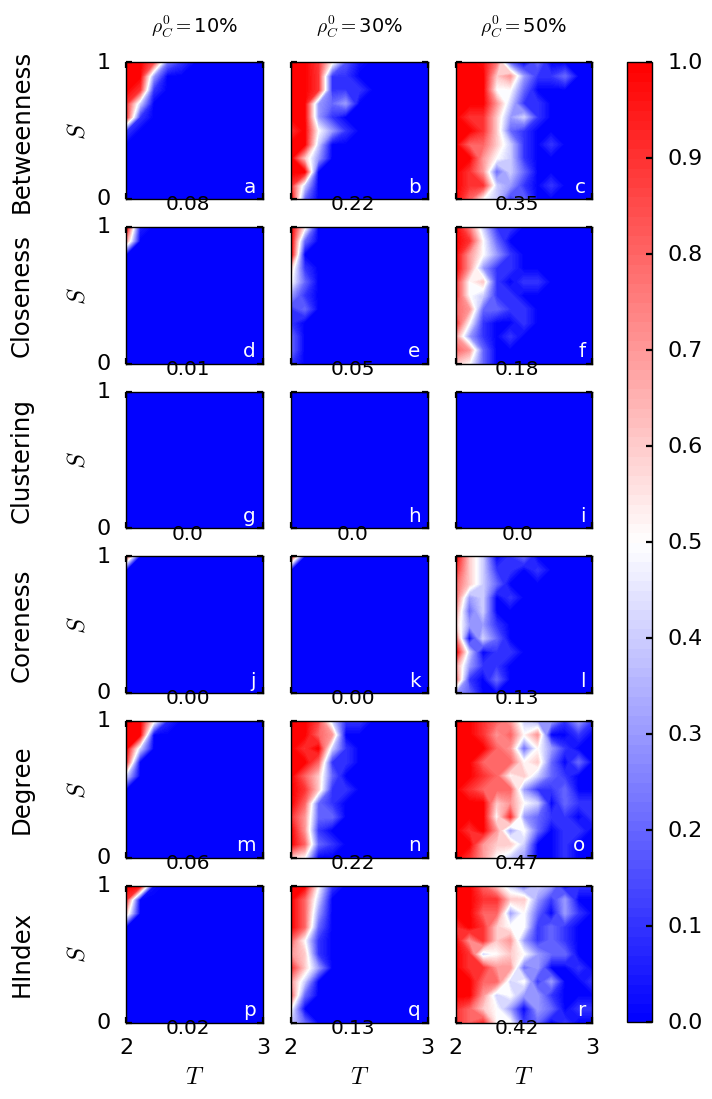
\includegraphics[width=13cm]{PowerlawK8RankUpdate.png}
\caption{Asymptotic density of cooperators $\mathcal{C}$ in degree $k=8$.
Other parameters are the same as in Fig.\ref{PowerlawK2RankUpdate}.}
\label{PowerlawK8RankUpdate}
\end{figure}


\begin{figure}[htbp]
\centering
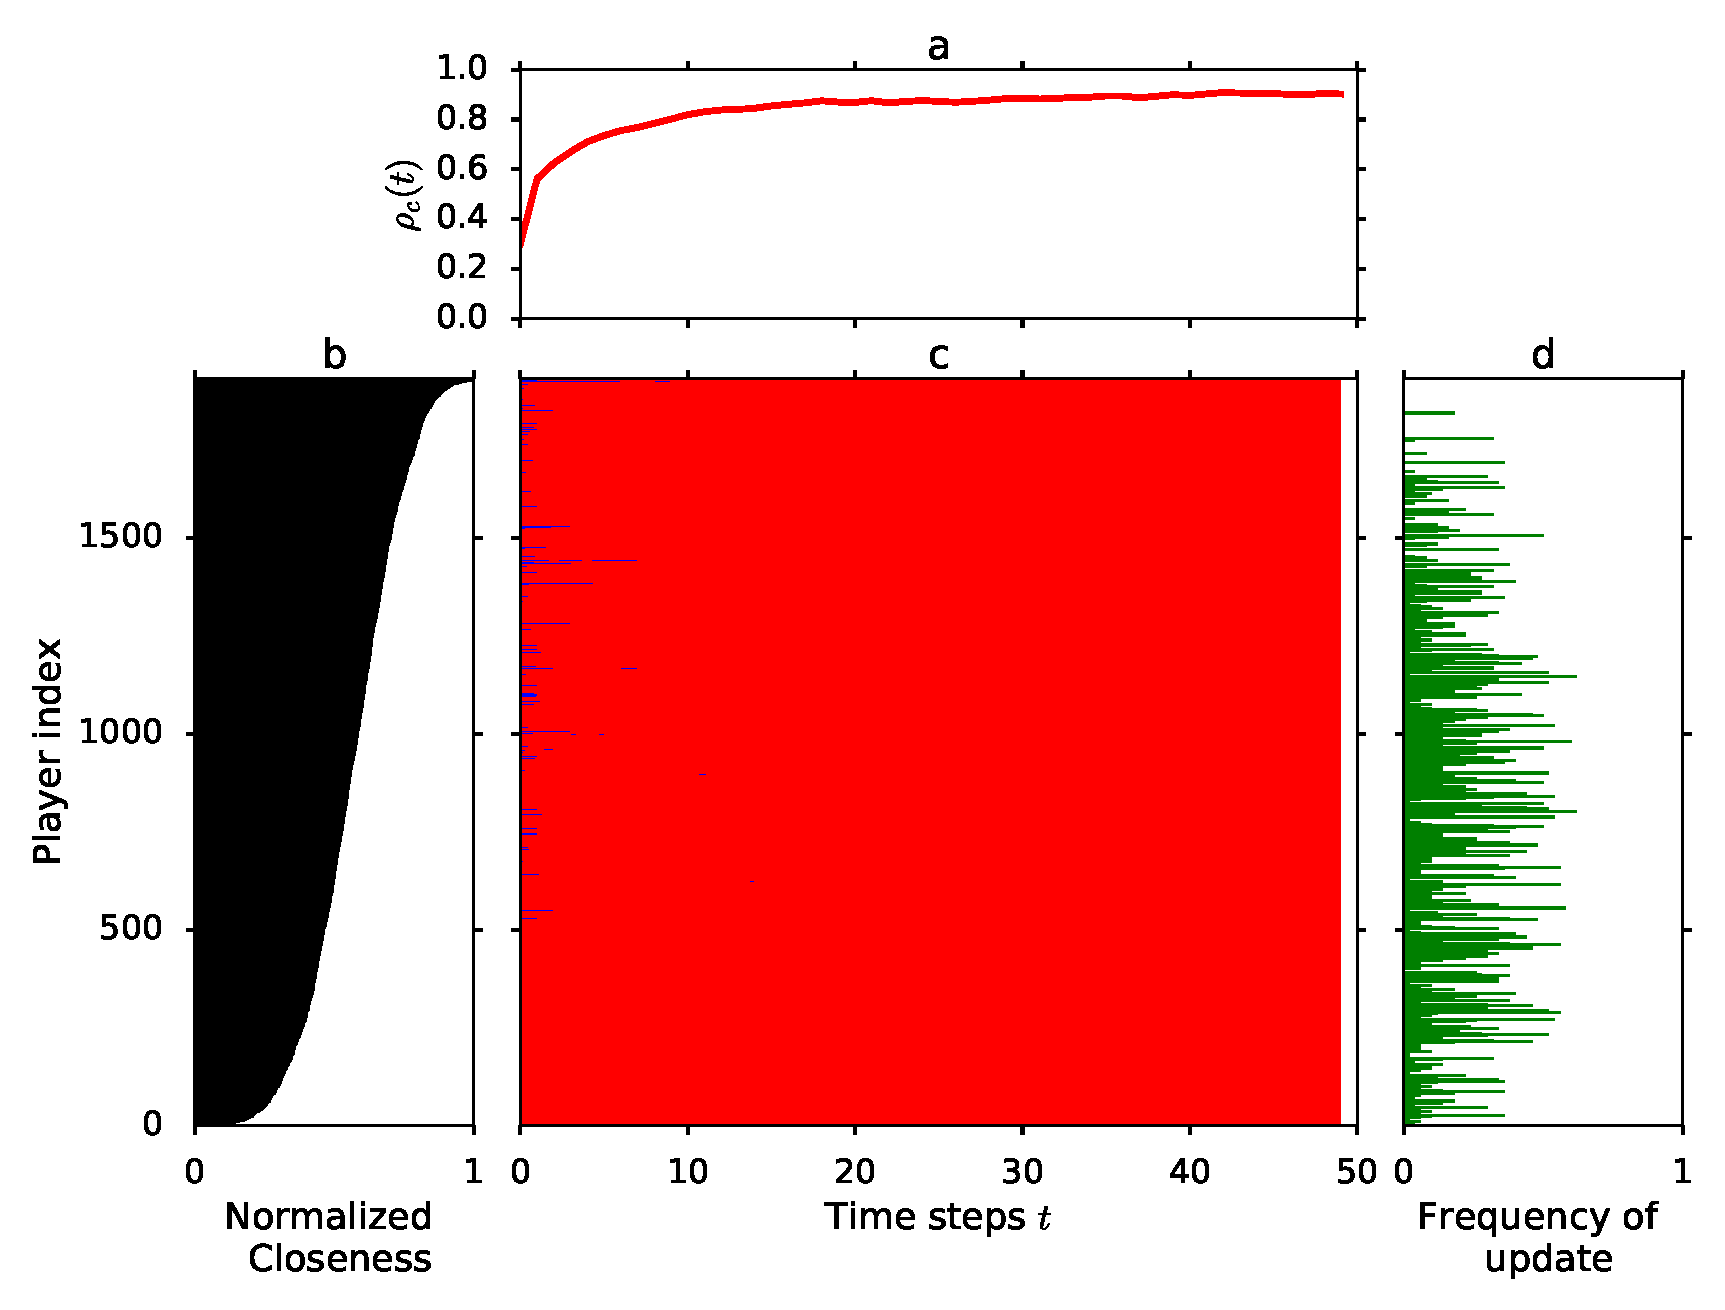
\includegraphics[width=13cm]{Powerlawk3PayoffUpdate.eps}
\caption{One realization of game with payoff update of strategy where cooperation level reaches
0.91 when $t=48$.
The game parameters used were $k=4,T=2.5,S=0.5,\rho_{C}(0)=0.3$ and centrality is Closeness.
(a) Cooperation level $\rho_{C}(t)$ varies with time step $t$.
(b) Normalized centrality of each player in descending order.
(c) The strategy adopted by each player at each time step.
(d) Frequency of updating strategy of each player during transient period(from $t=0$ to $t=T_{stable}$). }
\label{payoffUpdateProcess}
\end{figure}


\begin{figure}[htbp]
\centering
\includegraphics[width=13cm]{Powerlawk3centralityUpdate.eps}
\caption{One realization of game with mixed update of strategy where cooperation level decays
to zero when $t=1124$.
The game parameters are the same as in Fig.\ref{payoffUpdateProcess} and centrality is Closeness.
(a) Cooperation level $\rho_{C}(t)$ varies with time step $t$.
(b) Normalized centrality of each player in descending order.
(c) The strategy adopted by each player at each time step.
(d) Frequency of updating strategy of each player during transient period(from $t=0$ to $t=T_{stable}$). }
\label{centralityUpdateProcess}
\end{figure}

\begin{figure}[htbp]
\centering
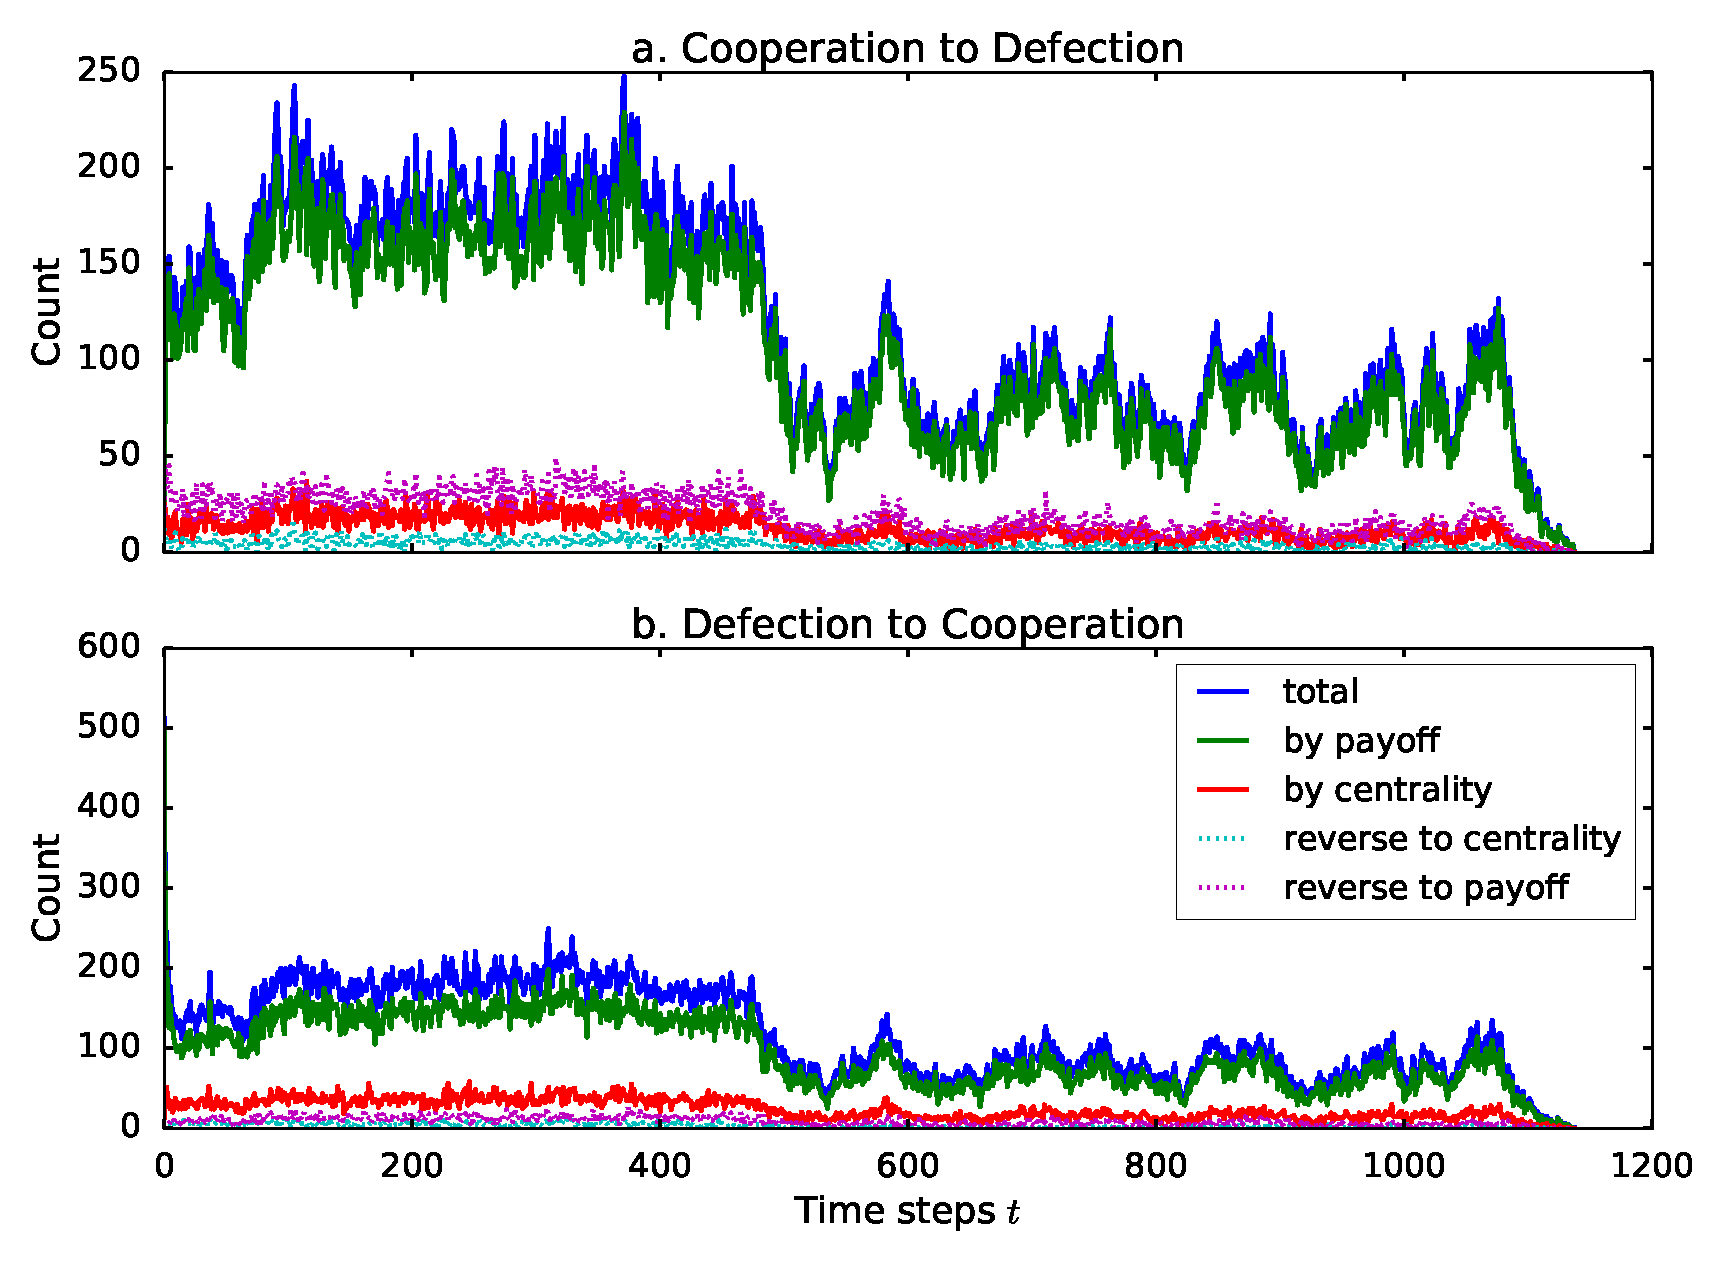
\includegraphics[width=10cm]{Powerlawk3centralityUpdateDetails.eps}
\caption{The process of updating strategy from cooperation to defection(a) and versa(b)
corresponding to Fig.\ref{centralityUpdateProcess}.
According to Eq.\ref{eq_mixedFermi}, a focal player updating strategy is probabilistically
determined by payoffs or by centralities.
 }
\label{centralityUpdateProcessDetails}
\end{figure}

%%%%%%%%%%%%%%%%%%%%%%%%%%%%%%%%%%%%%%%%%%%%%%%%%%%%%%%%%%%%%%%%%%%
\section{Conclusion}

    In order to explorer for this study the influences on the evolutionary outcome
caused by individual importance, we systematically analyzed the properties of aforementioned
centralities, including the distribution of centrality score and correlation.
   In short, investigate the effect of centrality in evolutionary game is important,
since a better understanding would allow controlling the evolutionary dynamic,
which for the scope of this paper, means exploring which individuals are
more closely related to cooperative behaviors.

In this work we have investigated the effect of individual importance on the evolution of cooperation.

To this end, we have considered a mechanism for players to update their strategy based on
the mixed comparison of payoff and centrality.


Besides centralities, the degree $k$ and initial fraction of cooperators $\rho_{C}(0)$
also have interconnected striking influence toward evolution outcome.

conclusion is strengthened and quantitatively corroborated
the non-monotonous variation of results across the ST-space

attenuate

Moreover, the impact of centrality correlated aspiration levels has also been studied [101], and it was shown that a positive correlation, such that the larger the degree of a player the higher its aspiration level, promotes cooperation. Together, these results indicate that favouring hubs by either decreasing their investments or increasing their pay-offs or aspiration promotes the evolution of public cooperation, which in turn strengthens the importance of hubs as declared already in the seminal paper by Santoset al.[90]. Social diversity promotes the emergence of cooperation in public goods games.

These results may help us understand questions such as how a network structure influences the evolutionary
process, how to design suitable collaboration networks and stimulate population to promote cooperative behaviors.

To conclude, we must recognize the strong dependence on details of evolutionary games on structured networks.
As a consequence, it does not seem plausible to expect general laws that could be applied in a wide range of practical situations.
On the contrary, a close modeling including the
kind of game, the evolutionary dynamics and the population structure of the concrete problem seems mandatory to reach sound and compelling conclusions.


%%%%%%%%%%%%%%%%%%%%%%%%%%%%%%%%%%%%%%%%%%%%%%%%%%%%%%%%%%%%
%% References with bibTeX database:

\bibliographystyle{elsarticle-num}
% \bibliographystyle{elsarticle-harv}
% \bibliographystyle{elsarticle-num-names}
% \bibliographystyle{model1a-num-names}
% \bibliographystyle{model1b-num-names}
% \bibliographystyle{model1c-num-names}
% \bibliographystyle{model1-num-names}
% \bibliographystyle{model2-names}
% \bibliographystyle{model3a-num-names}
% \bibliographystyle{model3-num-names}
% \bibliographystyle{model4-names}
% \bibliographystyle{model5-names}
% \bibliographystyle{model6-num-names}

\bibliography{references}

\end{document}

